\documentclass[lang=cn,10pt]{elegantbook}
\usepackage{graphicx}
\usepackage{float}

\title{热学}



\author{ Huang}
\date{\today}


\extrainfo{不要以为抹消过去,重新来过,即可发生什么改变。—— 比企谷八幡}

\setcounter{tocdepth}{3}


\cover{cover.jpg}

% 本文档命令
\usepackage{array}
\newcommand{\ccr}[1]{\makecell{{\color{#1}\rule{1cm}{1cm}}}}

% 修改标题页的橙色带
% \definecolor{customcolor}{RGB}{32,178,170}
% \colorlet{coverlinecolor}{customcolor}

\begin{document}
	
	\maketitle
	\frontmatter
	
	\tableofcontents
	
	\mainmatter
	\chapter{温度}
	\section{导学}
	这一章我们要求掌握的并不多,主要是几个基本的定义以及理想气体状态方程以及范德瓦尔斯方程的运用
	
	\section{前置知识}
	
	\begin{definition}[平衡态]
		在不受外界影响的条件下,一个热力学系统的宏观性质(温度、压强等)不随时间改变的状态,叫做平衡态
	\end{definition}
	
	我们需要重点掌握的定义就只有这个。接下来到公式部分。主要分为两种情况
	
	第一种是对理想气体使用的
	\begin{theorem}[理想气体状态方程]{理想}
		对于理想气体,我们有
		\begin{equation*}
			pV=\nu RT=\frac{m}{M}RT
		\end{equation*}
		其中$p,V,\nu,T,m,M$分别为系统的压强,体积,总物质的量,温度,总质量,平均摩尔质量,注意的是,代入计算时,
		$R\text{取}8.31\text{,}M\text{要乘上}10^{-3}\text{变化单位}
		$
	\end{theorem}
	
		另一种是对于非理想气体的
	\begin{theorem}[范德瓦尔斯方程]{非理想}
		对于非理想气体,我们有
		\begin{equation*}
			\left( p+\frac{m^2a}{M^2V^2} \right) \left( V-\frac{m}{M}b \right) =\frac{m}{M}RT
		\end{equation*}
		通常的,我们会取一摩尔的气体,方程简化为
		\begin{equation*}
			\left( p+\frac{a}{{V_m}^2} \right) \left( V-b \right) =RT
		\end{equation*}
	\end{theorem}
	\section{理想气体状态方程的应用}
	\begin{example}
		水银压强计中混入了一个空气泡,因此它的读数比实际的气压小.当精确的压强计的读数为768 mmHg时,它的读数只有748 mmHg,此时管内水银面到管顶的距离为80 mm,问当此压强计的读数为734 mmHg时,实际气压应该是多少?设空气的温度保持不变。
	\end{example}
	
	\begin{solution}
		分析:
		
		水银压强计的刻度是从上到下依次减小,在压强计的顶端是真空的,现在混入了一个空气泡,就让空气泡体积变大,就把我们的液体柱子往下压,造成了实际读数偏小
		
		首先我们对液体住上方的空气分析,气高度为80mm ,读数变小的数值就是实际气体压强的大小,故其压强为768-748=20 mmHg。现在其读数为743mmHg,此时空气柱的长度我们可以算出来,为80+748-734=94mm,然后只要我们算出其的压强,就可以求出外界的实际压强,在这一整个过程中,事实上,气体在做等温变化,于是乎,就有下述方程
		\begin{equation*}
			p_{1}V_{1}=p_{2}V_{2}
		\end{equation*}
		代入数据,可得
		\begin{equation*}
			20\times 80=94\times p_{2}
		\end{equation*}
		解得
		\begin{equation*}
			p_{2}=17.02mmHg
		\end{equation*}
		于是乎,实际气压为
		\begin{equation}
			p=p_{2}+734=751.02Hg
		\end{equation}
		\end{solution}
	~\\
	
	\begin{example}
		$
		\text{一打气筒,每打一次气可将原来压强为}p_0=1.0 atm\,\,,\text{温度为}t_0=-3.0$℃$\text{,}
		\\
		\text{体积}V_0=4.0 L\text{的空气压缩到容器内,设容器的体积为}V=1.5\times 10^3L,\text{问}
		\\
		\text{需要打几次气,才能使容器的空气温度为}t=45$℃$\text{,压强为}p_0=2.0 atm
		$
	\end{example}
	\begin{solution}
		将气体温度转化为开氏温度,有$t_{0}$=270K,$t$=318K
		
		对于理想气体,我们有
		\begin{equation*}
			pV=\nu RT=\frac{m}{M}RT
		\end{equation*}
		打一次气,我们打进去的质量$\varDelta m$为
		\begin{equation}
			\varDelta m=\frac{p_0V_0M}{RT_0}
		\end{equation}
		对于结果中的气体质量$m$,我们有
		\begin{equation*}
			m=\frac{pVM}{RT}
		\end{equation*}
		则我们打气的次数$n$为
		\begin{equation*}
			n=\frac{m}{	\varDelta m}=\frac{pVT_{0}}{p_0V_0T}
		\end{equation*}
		\begin{equation*}
			n=636.79
		\end{equation*}
		由于我们只能多打,不能少打,就有
		\begin{equation*}
			n=637
		\end{equation*}
	\end{solution}
	~\\
	\begin{example}
		按重量计,空气是由76$\%$的氨,23$\%$的氧,约1$\%$的氩组成的,试求空气的平均相对分子质量以及在标况下的密度。
	\end{example}
	
	\begin{solution}
		对于理想气体,我们有
		\begin{equation*}
			pV=\nu RT=\frac{m}{M}RT
		\end{equation*}
		左右两边同除$V$,就有
		\begin{equation*}
			pM=\rho RT
		\end{equation*}
		于是乎,我们就有以下密度公式
		\begin{equation}
			\rho=\frac{pM}{RT}
		\end{equation}
		由于温度,压强为已知的,我们要求出气体的密度,只要求出气体的平均摩尔质量$\overline{M}$即可
		考虑到
		\begin{equation*}
			\frac{m_{\text{总}}}{\overline{M}}=n_{\text{总}}
		\end{equation*}
		我们设氮气的质量为$m_{1}$,氧气的质量为$m_{2}$,氩气的质量为$m_{3}$
		
		就有
		\begin{equation*}
			\frac{m_{\text{总}}}{\overline{M}}=\frac{m_{1}}{M_{1}}+\frac{m_{2}}{M_{2}}+\frac{m_{3}}{M_{3}}
		\end{equation*}
		我们取$m_{\text{总}}$=100,则有
		\begin{equation*}
			\frac{100}{\overline{M}}=\frac{76}{M_{1}}+\frac{23}{M_{2}}+\frac{1}{M_{3}}
		\end{equation*}
		解得
		\begin{equation*}
			\overline{M}=28.9\times 10^{-3} kg\cdot mol^{-1}
		\end{equation*}
		代入密度公式,就有
		\begin{equation*}
			\rho =1.29\times 10^{-3}kg\cdot L^{-1}
		\end{equation*}
	\end{solution}
	
	\section{范德瓦尔斯方程的应用}
	
	\begin{example}
		1 mol氧气,压强为1000atm,体积为0.050L,其温度为多少?
	\end{example}
	\begin{solution}
		对1mol的非理想气体,由范德瓦尔斯方程可得
		\begin{equation*}
			\left( p+\frac{a}{{V_m}^2} \right) \left( V-b \right) =RT
		\end{equation*}
		对于氧气$a=1.360atm\cdot L^{2} \cdot mol^{-2},b=0.03183L\cdot mol^{-1}$,代入计算,可达
		\begin{equation*}
			T=342.1K
		\end{equation*}
	\end{solution}
	\chapter{气体分子动理论}
	\section{导学}
		这一章节,我们要注意的是一个速率和两个公式,然后由上一节内容推出的范德瓦尔斯气体的压强我们蛮注意一下,有的膈应人的题目会考。
	\section{前置知识}
	
	首先我们来到一个速率,也就是分子的方均根速率
	
	\begin{definition}[方均根速率]
		我们定义大量气体分子速率的平方的平均值的平方根为方均根速率,其形式如下
		\begin{equation*}
			\sqrt{\overline{v^2}}=\sqrt{\frac{3kT}{m}}=\sqrt{\frac{3RT}{M}},\text{其中}k=\frac{R}{N_{A}}=1.38\times10^{-23}J/K
		\end{equation*}
	\end{definition}
	
	然后我们来到两个公式中的第一个
	\begin{theorem}[平均平动动能公式]
		\begin{equation*}
			\overline{\varepsilon }=\frac{3}{2}kT,\text{其中}k=\frac{R}{N_{A}}=1.38\times10^{-23}J/K
		\end{equation*}
		这个公式表明,气体的平均平动动能只与温度有关,并且成正比。
	\end{theorem}
	
	然后就是用的比较多的压强公式
	\begin{theorem}[压强公式]
		\begin{equation*}
			p=nkT,k=\frac{R}{N_{A}}=1.38\times10^{-23}J/K,n\text{为分子数密度}
		\end{equation*}
	\end{theorem}
	接下来的结论,我们了解即可
	\begin{theorem}[范德瓦尔斯气体压强]{非理想压强}
		通常的,我们会取一摩尔的气体
		\begin{equation*}
			p=\frac{RT}{V_m-b}-\frac{a}{V_{m}^{2}}
		\end{equation*}
		其中$V_{m}$是1mol气体的体积,a,b是由气体性质确定的常量。
	\end{theorem}
	
	\section{两个公式的应用}
	\begin{example}
		钠黄光的波长为589.3nm。设想一立方体每边长$L=$5.893$\times 10 ^{-7}$m,试问在标况下其中有多少个空气分子。
	\end{example}
	\begin{solution}
		我们要求出标况下已知体积大小的钠的数量,只需要求其分子数密度再与体积相乘即可得到对应的分子数,此时我们已经知道标况下的温度和气体压强,所以我们有以下公式
		\begin{equation*}
			p_{0}=nkT
		\end{equation*}
		代入,我们可求得分子数密度
		\begin{equation*}
			n=\frac{p_{0}}{kT}
		\end{equation*}
		代入数值,解得
		\begin{equation*}
			n=2.89\times10^{25}m^{-3}
		\end{equation*}
		所以分子数$N$为
		\begin{equation*}
			N=nL^{3}
		\end{equation*}
			带入数值,可得
		\begin{equation*}
			N=5.50\times10^{6}
		\end{equation*}
	\end{solution}
	
	\begin{example}
		一容器内储有氧气,其压强为$p=1.01\times 10^{5}Pa$,温度为t=27℃求:
		
		(1)单位体积内分子数
		
		(2)氧气的密度
		
		(3)氧分子的质量
		
		(4)分子间的平均距离
		
		(5)分子的平均动能
	\end{example}
	\begin{solution}
		(1)此时我们已经知道压强和温度,我们有以下公式
		\begin{equation*}
			p=nkT
		\end{equation*}
		带入数值,解得
		\begin{equation*}
			n=2.45\times10^{25}m^{-3}
		\end{equation*}
		
		(2)对于求密度,我们有密度公式
		\begin{equation*}
			pM=\rho RT
		\end{equation*}
		代入数值,解得
		\begin{equation*}
			\rho=1.29\times 10^{-3}kg\cdot L^{-1}
		\end{equation*}
		
		(3)要求一个氧分子的质量$m$,我们只需要求1mol氧分子的质量再将其除以阿伏伽德罗常数$N_{A}$即可,就有以下方程
		\begin{equation*}
			m=\frac{M_{O_{2}}}{N_{A}}
		\end{equation*}
		代入数据,解得
		\begin{equation*}
			m=5.3\times 10^{-26}kg
		\end{equation*}
		
		(4)我们将氧分子视为正方体,其边长为$L$,视单位体积内中有n个氧分子,那么单位体积的数值与n个小正方体的体积相同,则有
		\begin{equation*}
			1=nL^{3}
		\end{equation*}
		代入之前的数据,解得
		\begin{equation*}
			L=3.47\times 10^{-9}m
		\end{equation*}
		
		(5)看到平均动能,我们考虑平均动能公式
		\begin{equation*}
			\overline{\varepsilon }=\frac{3}{2}kT
		\end{equation*}
		代入数据,解得
		\begin{equation*}
			\overline{\varepsilon }=6.21\times10^{-21}J
		\end{equation*}
	\end{solution}
	
	\chapter{气体分子热运动速率和能量的统计分布律}
	\section{导学}
	这一章考点很多,很密集,主要是围绕麦克斯韦速率分布函数,然后由其进行衍生,扩展
	\section{前置知识}
	
	 为了研究目标物体速度变化的快慢,我们引进了加速度的概念,类比一下,我们为了研究某个事件发生的概率与区间的变化的关系,进而引进了概率分布函数,若这个事件的区间是速率,则我们又称这个函数为速率分布函数
	 
	 \begin{definition}[速率分布函数]
	 	我们定义以下为速率分布函数:
	 	\begin{equation*}
	 		f\left( v \right) dv=\frac{dN}{N}
	 	\end{equation*}
	 	其图像的几何意义就是气体落在某个区间的概率
	 	
	 	经过严谨的数学推导,其形式如下:
	 	\begin{equation*}
	 		f\left( v \right) =4\pi v^2\left( \frac{m}{2\pi kT} \right) ^{\frac{3}{2}}e^{-\frac{mv^2}{2kT}}
	 	\end{equation*}我们又称之为麦克斯韦气体速率分布函数
	 \end{definition}
	 
	 根据这个几何意义,我们自然就有以下结论
	 
	 \begin{conclusion}
	 	\begin{equation*}
	 		\int\limits_0^{\infty}{f\left( v \right) dv}=1
	 	\end{equation*}
	 \end{conclusion}
	 我们称之为\textbf{归一化}。
	 
	 这个问题解决之后,我们就来到一个重要的知识点——三个速率
	 
	 \begin{definition}[三个速率]
	 	我们称$f(v)$的极大值对应的速率为\textbf{最该然速率},其形式如下
	 	\begin{equation*}
	 		v_p=\sqrt{\frac{2kT}{m}}=\sqrt{\frac{2RT}{M}},\text{其中}k=\frac{R}{N_{A}}=1.38\times10^{-23}J/K
	 	\end{equation*}
	 	主要在讨论分子的速率分布时用。
	 	
	 	我们定义大量分子速率的算数平均值为分子的平均速率,其形式如下
	 	\begin{equation*}
	 		\overline{v}=\sqrt{\frac{8kT}{\pi m}}=\sqrt{\frac{8RT}{\pi M}},\text{其中}k=\frac{R}{N_{A}}=1.38\times10^{-23}J/K
	 	\end{equation*}
	 	主要在讨论分子碰撞问题时用。
	 	
	 	我们定义大量气体分子速率的平方的平均值的平方根为\textbf{方均根速率},其形式如下
	 	\begin{equation*}
	 		\sqrt{\overline{v^2}}=\sqrt{\frac{3kT}{m}}=\sqrt{\frac{3RT}{M}},\text{其中}k=\frac{R}{N_{A}}=1.38\times10^{-23}J/K
	 	\end{equation*}
	 	主要在讨论分子平均平动动能时用。
	 \end{definition}
	 
	 有了最该然速率之后,我们就可以对麦克斯韦速率分布函数进行化简。形式如下
	 
	 	\begin{equation*}
	 		\text{令}u=\frac{v}{v_p}\text{,就有}
	 		\frac{dN}{N}=\frac{4}{\sqrt{\pi}}e^{-u^2}u^2du
	 		,\varDelta u\text{很小时候,}du\approx \varDelta u,
	 		\text{原式等价于}\frac{\varDelta N}{N}=\frac{4}{\sqrt{\pi}}e^{-u^2}u^2\varDelta u
	 	\end{equation*}

	接下来一个知识点,挺有趣的,大家当成结论记住吧
	
	\begin{theorem}[单位碰壁分子数]
		在单位时间碰到单位面积器壁上的气体分子数为
		\begin{equation*}
			\frac{1}{4}n \bar{v}
		\end{equation*}
	\end{theorem}
	这个结论我们在后续会用到。
	
	目前为止,麦克斯韦气体速率分布的内容就结束了,由于涉及到能量的部分分配也仅仅是对于平均平动动能的分配,接下来我们要考虑对另一种能量的,也就是对势能的分配,即\textbf{玻尔兹曼分布律}
	
	\begin{definition}[玻尔兹曼分布律]
		我们将分子按势能分布的分布律叫做玻尔兹曼分布律,形式如下
		\begin{equation*}
			n=n_{0}e^{-\frac{\varepsilon _p}{kT}}
		\end{equation*}
	\end{definition}
	
	设在高度为z=0的地方单位体积内分子数为$n_{0}$我们能立即得到以下结论
	\begin{conclusion}
		分布在高度z处单位体积内的分子数为
		\begin{equation*}
			n=n_{0}e^{-\frac{mgz}{kT}}
		\end{equation*}
	\end{conclusion}
	
	由此,我们能得到一个等温气压公式
	\begin{theorem}[等温气压公式]
		设气体在高度z=0的压强为$p_{0}$,则在高度z=z处有
		\begin{equation*}
			p=p_{0}e^{-\frac{mgz}{kT}}=p_{0}e^{-\frac{Mgz}{RT}}
		\end{equation*}
		取对数后,还可以变成
		\begin{equation*}
			z=\frac{RT}{Mg}\ln \frac{p_0}{p}
		\end{equation*}
	\end{theorem}
	
	接下来,我们要来到一个经常考的部分——能量按自由度分配
	
	\begin{theorem}[能均分定理]
		在温度为T的平衡状态下,物质分子的每一个自由度都具有相同的平均动能,其大小都等于$\frac{1}{2}kT$,设某种气体气体的平动自由度为t,转动自由度为r,振动自由度为s,则分子的平均总动能为$\frac{s+r+t}{2}kT$
	\end{theorem}
	
	由于分子的内能是分子的动能加上分子内部之间的势能,则对于1mol理想气体,其内能为
	\begin{equation*}
		\frac{2s+r+t}{2}RT
	\end{equation*}
	因此,对于单原子气体,其内能等于
	\begin{equation*}
		\frac{3}{2}RT
	\end{equation*}
	
	对于双原子分子气体,其内能等于
	 \begin{equation*}
	 	\frac{7}{2}RT
	 \end{equation*}
	 
	 现在,我们来到理想气体的热容。
	 
	 \begin{definition}[摩尔热容]
	 	1mol物质升高或降低1$℃$所吸收(放出)的热量叫做物质的摩尔热容记作$C_{m}$
	 \end{definition}
	 现在我们增添一个体积不变的条件,则其为变为定容摩尔热容记为$C_{V,m}$
	 由摩尔热容的定义,则可有下列式子
	 \begin{equation*}
	 	C_{V,m}=\frac{2s+r+t}{2}R
	 \end{equation*}
	 这里我们要注意的是,虽然双原子分子气体的摩尔热容为$\frac{7}{2}R $,但事实上,在只有几百k的时候,其摩尔热容只有$\frac{5}{2}R$,这个在第五章用的很多。
	 
	\section{三个速率习题}
	\begin{example}
		试计算300K下的氧气分子的三种速率
	\end{example}
	\begin{solution}
		最概然速率如下
		\begin{equation*}
			v_{p}=\sqrt{\frac{2kT}{m}}=\sqrt{\dfrac{2RT}{M}}
		\end{equation*}
		代入数据,解得
		\begin{equation*}
				v_{p}=3.95\times10^{2}m/s
		\end{equation*}
		平均速率如下
		如下
		\begin{equation*}
			\overline{v}=\sqrt{\frac{8kT}{\pi m}}=\sqrt{\dfrac{8RT}{\pi M}}
		\end{equation*}
		代入数据,解得
		\begin{equation*}
			\overline{v}=4.46\times10^{2}m/s
		\end{equation*}
		方均根速率如下
		\begin{equation*}
			\sqrt{\overline{v^2}}=\sqrt{\frac{3kT}{m}}=\sqrt{\dfrac{3RT}{M}}
		\end{equation*}
		代入数据,解得
		\begin{equation*}
			\sqrt{\overline{v^2}}=4.83\times10^{2}m/s
		\end{equation*}
	\end{solution}
	
	\section{麦克斯韦气体速率分布函数习题}
	\begin{example}
		设氢气的温度为300℃,求速率在3000 m/s 到 3010m/s之间的分子数$\varDelta N_{1}$与速率在1500m/s到1510m/s之间的分子数$\varDelta N_{2} $之比
	\end{example}
	\begin{solution}
		我们首先考虑麦克斯韦气体速率分布函数
		\begin{equation*}
			f\left( v \right) =4\pi v^2\left( \frac{m}{2\pi kT} \right) ^{\frac{3}{2}}e^{-\frac{mv^2}{2kT}}
		\end{equation*}
		由函数的几何意义,我们可以知道
		\begin{equation*}
			\begin{split}
				\varDelta N_{1}=N\int\limits_{3000}^{3010}{f\left( v \right) dv}
				\\
				\varDelta N_{2}=N\int\limits_{1500}^{1510}{f\left( v \right) dv}
			\end{split}
		\end{equation*}
		当积分的上下界相差很小的时候,我们可以做近似计算,即
		\begin{equation*}
			N\int\limits_v^{v+\varDelta v}{f\left( v \right) dv}\approx Nf\left( v \right) \varDelta v
		\end{equation*}
		因此
		\begin{equation*}
			\begin{split}
				\varDelta N_{1}=N\int\limits_{3000}^{3010}{f\left( v \right) dv}=Nf\left( v_{1} \right) \varDelta v
				\\
				\varDelta N_{2}=N\int\limits_{1500}^{1510}{f\left( v \right) dv}=Nf\left( v_{2} \right) \varDelta v
			\end{split}
		\end{equation*}
		则有
		\begin{equation*}
			\frac{\varDelta N_{1}}{\varDelta N_{2}}=\frac{f\left( v_{1} \right)}{f\left( v_{2} \right)}=\left( \frac{v_1}{v_2} \right) ^2e^{-\frac{m\left( v_{1}^{2}-v_{2}^{2} \right)}{2kT}}=\left( \frac{v_1}{v_2} \right) ^2e^{-\frac{M\left( v_{1}^{2}-v_{2}^{2} \right)}{2RT}}
		\end{equation*}
		代入数据可得
		\begin{equation*}
			\frac{\varDelta N_{1}}{\varDelta N_{2}}\approx0.9692
		\end{equation*}
	\end{solution}
		
	\begin{example}
		已知容积为V的容器内部压强$p_{0}$远大于外界的压强,$T=const$,求当出现面积为$A$的小孔时候,气体压强泄漏到原来一半所用的时间。
	\end{example}
	\begin{solution}
		我们要求出气体泄漏的速度,就要求出单位时间内与小孔发生碰撞的气体分子数
		对于单位时间与单位面积发生碰撞的气体分子数$N$,我们有
		\begin{equation*}
			N=\frac{1}{4}n\overline{v}
		\end{equation*}
		我们分析在$dt$时间内所发生碰撞的分子$dN$,设此时气体分子数为$N$,有
		\begin{equation*}
			dN=\frac{1}{4}n\overline{v}Adt=\frac{1}{4}\frac{N}{V}\overline{v}Adt
		\end{equation*}
		我们要将其与压强联系,考虑到压强公式
		\begin{equation*}
			p=nkT=\frac{N}{V}kT
		\end{equation*}
		两边同取微分,可得
		\begin{equation*}
				dp=d\frac{N}{V}kT
		\end{equation*}
		代入原式,可得
		\begin{equation*}
			\frac{Vdp}{kT}=\frac{1}{4}\frac{N}{V}\overline{v}Adt
		\end{equation*}
		化简可得
		\begin{equation*}
			\frac{Vdp}{NkT}=\frac{dp}{\frac{N}{V}kT}=\frac{dp}{p}=\frac{1}{4}\frac{1}{V}\overline{v}Adt
		\end{equation*}
		对等式两边同时积分,有
		\begin{equation*}
			\int\limits_{p_0}^{\frac{p_0}{2}}{}\frac{dp}{p}=\int\limits_0^t{}\frac{1}{4}\frac{1}{V}\overline{v}Adt
		\end{equation*}
		解得
		\begin{equation*}
			t=\frac{4V}{\overline{v}A}\ln2
		\end{equation*}
	\end{solution}
	~\\
	\begin{example}
		一容器被隔板分离为两部分,其中气体的压强,分子数密度分别为$p_{1},n_{1},p_{2},n_{2}$.两部分气体的温度相同,都等于T,摩尔质量也相同,均为M,试证明:如隔板上有一面积为$A$的小孔,则每秒通过小孔的气体质量为
		\begin{equation*}
			m=\sqrt{\frac{M}{2\pi RT}}A\left( p_1-p_2 \right) 
		\end{equation*}
	\end{example}
	\begin{solution}
		我们要求每秒通过小孔的气体质量,即要求单位时间内通过单位面积的气体分子数$N$,然后再化为mol单位,乘以摩尔质量即可
		对于单位时间内从左边到右边的分子数,我们有
		\begin{equation*}
			N_{1}=\frac{1}{4}n_{1}\overline{v}A
		\end{equation*}
		对于单位时间内从右边到左边的分子数,我们有
		\begin{equation*}
			N_{2}=\frac{1}{4}n_{2}\overline{v}A
		\end{equation*}
		于是单位时间内总共从左向右迁移的气体分子数$\varDelta N$为(不妨假设左边大于右边)
		\begin{equation*}
			\varDelta N=N_{1}-N_{2}=\frac{1}{4}(n_{1}-n_{2})\overline{v}A
		\end{equation*}
		然后化为mol,求出每秒净从左到右的气体质量$m$
		\begin{equation*}
			m=\frac{1}{4}(n_{1}-n_{2})\overline{v}A\frac{M}{N_{A}}
		\end{equation*}
		接着我们要观察结论形式,发现里面有压强没有分子数密度,并且没有平均速率,故考虑以下公式对其代换
		\begin{equation*}
			p=nkT,	\overline{v}=\sqrt{\frac{8kT}{\pi m}}=\sqrt{\dfrac{8RT}{\pi M}}
		\end{equation*}
		代入后,解得
		\begin{equation*}
			m=\sqrt{\frac{M}{2\pi RT}}A\left( p_1-p_2 \right)
		\end{equation*}
		
	\end{solution}
	~\\
	\begin{example}
		N个假想的气体分子,其速率分布入图3.1所显示,求
		% TODO: \usepackage{graphicx} required
		\begin{figure}[H]
			\centering
			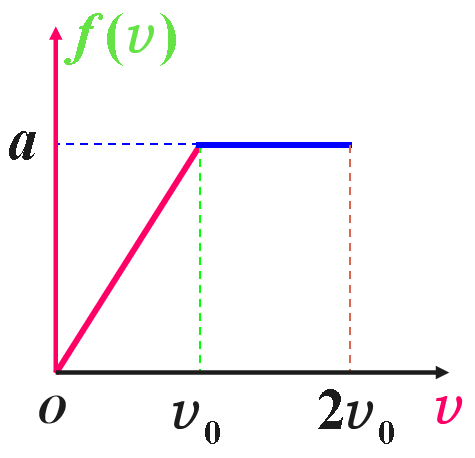
\includegraphics[width=0.2\linewidth]{screenshot003}
			\caption{}
			\label{fig:screenshot003}
		\end{figure}
		
		(1)a(用N和$v_{0}$表示)
		
		(2)速率在1.5$v_{0}$和$2.0v_{0}$之间的分子数
		
		(3)求分子的平均速率
	\end{example}
	\begin{solution}
		(1)由归一化条件,函数的图像面积和为1
		则有
		\begin{equation*}
			N\frac{a(v_{0}+2v_{0})}{2}=1
		\end{equation*}
		解得\begin{equation*}
			a=\frac{2N}{3v_{0}}
		\end{equation*}
		
		(2)由麦克斯韦气体速率分布函数图像的几何意义,速率在1.5$v_{0}$和$2.0v_{0}$之间的分子数为
		\begin{equation*}
			\int\limits_{1.5v_0}^{2v_{0}}{Nf\left( v \right) dv}=\frac{N}{3}
		\end{equation*}
		
		(3)根据气体平均速率的定义,有
		\begin{equation*}
			\overline{v}=\int\limits_{0}^{2v_{0}}{vf\left( v \right) dv}=\frac{11}{9}v_{0}
		\end{equation*}
	\end{solution}
	
	\begin{example}
		根据麦克斯韦气体速率分布,求速率倒数的平均值$\overline{\frac{1}{v}}$
	\end{example}
	\begin{solution}
		根据定义有
		\begin{equation*}
			\overline{\frac{1}{v}}=\int\limits_0^{\infty}{\frac{1}{v}f\left( v \right) dv}
		\end{equation*}
		又因为
		\begin{equation*}
			f\left( v \right) =4\pi v^2\left( \frac{m}{2\pi kT} \right) ^{\frac{3}{2}}e^{-\frac{mv^2}{2kT}}
		\end{equation*}
		代入可得
		\begin{equation*}
			\overline{\frac{1}{v}}=4\pi \left( \frac{m}{2\pi kT} \right) ^{\frac{3}{2}}\int\limits_0^{\infty}{ve^{-\frac{mv^2}{2kT}}dv}
		\end{equation*}
		由数学的凑微分技巧,我们可以算得结果为
		\begin{equation*}
			\overline{\frac{1}{v}}=\frac{4}{\pi}\sqrt{\frac{\pi m}{8kT}}
		\end{equation*}
	\end{solution}

	
	\section{微粒按高度分布习题}
	
	\begin{example}
		飞机的起飞前,机舱的压强计指示为1.0 atm,温度为27℃;起飞后,压强计指示为0.80atm,温度仍为27摄氏度,试计算飞机距地面的高度,若当前的温度为0℃,上升到什么高度处压强减为地面的75$\%$?	
	\end{example}
	\begin{solution}
		我们取地面为$z=0$处,对气体列等温气压公式,有
		\begin{equation*}
			p=p_{0}e^{-\frac{mgz}{kT}}=p_{0}e^{-\frac{Mgz}{RT}}
		\end{equation*}
		取对数后,有
		\begin{equation*}
			z=\frac{RT}{Mg}\ln \frac{p_0}{p}
		\end{equation*}
		代入数据,解得
		\begin{equation*}
			z=1.96\times10^{3}m
		\end{equation*}
	\end{solution}
	\section{能均分定理习题}
	\begin{example}
		在室温300K下,1mol氢和1mol氮的内能各是多少?1g氢和1g氮的内能各是多少?
	\end{example}
	\begin{solution}
		在室温下,这两个分子都为双原子分子,总自由度为5,由内能公式
		\begin{equation*}
			u=\frac{5}{2}RT
		\end{equation*}
		解得
		\begin{equation*}
			u=6.23\times10^{3}J\cdot mol^{-1}
		\end{equation*}
		由于氢和氮的相对分子量不同,故各自1g的内能不一样
		
		对于氢,有
		\begin{equation*}
			u_{1}=u\frac{1}{M_{1}}
		\end{equation*}
		代入数据,解得
		\begin{equation*}
				u_{1}=3.12\times10^{3}J\cdot mol^{-1}
		\end{equation*}
		
		对于氮,有
		\begin{equation*}
			u_{2}=u\frac{1}{M_{2}}
		\end{equation*}
		代入数据,解得
		\begin{equation*}
			u_{2}=2.2\times10^{2}J\cdot mol^{-1}
		\end{equation*}
	\end{solution}
	
	\begin{example}
		求常温下质量为$m_{1}=$3.00g的水蒸气与$m_{2}=$=3.00g的氢气的混合气体的定比热容
	\end{example}
	\begin{solution}
		我们设水蒸气的比定热容为$c_{V_{1}}$,氢气的比定热容为$c_{V_{2}}$设混合气体的比定热容为$c_{V_{3}}$,设升温$\varDelta T$,有
		\begin{equation*}
			c_{V_{3}}(m_{1}+m_{2})\varDelta T=(c_{V_{1}}m_{1}+c_{V_{2}}m_{2})\varDelta T
		\end{equation*}
		消去$\varDelta T$,有
		\begin{equation*}
			c_{V_{3}}(m_{1}+m_{2})=c_{V_{1}}m_{1}+c_{V_{2}}m_{2}
		\end{equation*}
		在常温下,水的定容摩尔热容为$3R$,氢气的定容摩尔热容为$\frac{5}{2}R$。
		又因为比定容容热容,满足$c_{v}=\frac{C_{V}}{m}=\frac{C_{V,m}}{M}$($N$为分子数)则有
		\begin{equation*}
			c_{V_{1}}=\frac{3R}{M_{1}},c_{V_{2}}=\frac{5R}{2M_{2}}
		\end{equation*}
		代入原式子,可得
		\begin{equation*}
			c_{V_{3}}=5.83J\cdot g^{-1}\cdot K^{-1}
		\end{equation*}
		
		\end{solution}
	\chapter{气体内的运输过程}
	\section{导学}
	这一章的内容不是很多,主要是对平均自由程的理解和对那三个系数的记忆,至于那三个系数怎么来的,就没什么必要掌握了。
	\section{前置知识}
	我们知道,气体分子总似在做无规则的运动,为了研究气体之间的碰撞,我们就得想办法确定气体发生碰撞所需的平均路程,于是,平均自由程相应而生
    \begin{definition}[平均自由程]
    	气体分子在相继两次碰撞所通过的路程的平均值为平均自由程,记为$\lambda$。其与分子的平均速率$\overline{v}$,碰撞频率$Z$的关系为
    	\begin{equation*}
    		\lambda=\frac{\overline{v}}{Z}
    	\end{equation*}
    	其与分子数密度$n$,分子有效直径$d$,温度$T$和压强$p$的关系为
    	\begin{equation*}
    		\lambda=\frac{1}{\sqrt{2}\pi d^{2}n}=\frac{kT}{\sqrt{2}\pi d^{2}p}
    	\end{equation*}
    \end{definition}
    \begin{note}
    	平均自由程与分子数密度$n$,分子有效直径$d$,温度$T$和压强$p$的关系的推导是这样的,我们是从这个公式出发
    	\begin{equation*}
    		\lambda=\frac{\overline{v}}{Z}
    	\end{equation*}
    	现在我们的目的就是求出碰撞频率。由于气体分子都是在运动的,所以我们要用相对运动来研究,其相对速度$v_{\text{相}}$满足以下关系
    	\begin{equation*}
    		v_{\text{相}}=\sqrt{2}\overline{v}
    	\end{equation*}
    	于是乎,我们取在很小的一段时间$\varDelta t$,如果在这一段时间发生碰撞的总分子数为$N$,碰撞的频率就是$\frac{N}{\varDelta t}$,下面我们求$N$,在这一小段时间内,气体分子移动的体积可近似看作小圆柱体,高为$v_{\text{相}\varDelta t}$,底面积为分子的碰撞截面,则分子总数为
    	\begin{equation*}
    		N=\sqrt{2}\pi d^{2}n \varDelta t
    	\end{equation*}
    	最后再代入第一个公式就可计算出来。
    \end{note}
    另外,平均自由程的大小与给定长度区间有关,其分子的数量,路程和平均自由程的大小满足
    \begin{equation*}
    	-\frac{dN}{N_0}=\frac{1}{\lambda}e^{-\frac{x}{\lambda}}dx,(\text{其中}N_{0}\text{为总分子数})
    \end{equation*}
    
    从平均自由程出发,我们就可以推导出三个现象以及其对应的系数,这三个系数是我们要记住的。
    
    
    \begin{definition}[黏性现象]
    	当气体各层流速不同时,通过任一平行于流速的截面,相邻两部分气体将沿平行于截面方向互施作用力,结果使得流动慢的气层加速,使流动快的气层减速。这种相互作用力称为内摩擦力,也叫做黏性力。这种现象称为内摩擦现象,也叫做\textbf{黏性现象}。其中在$dt$时间内,粘性力的冲量满足
    	\begin{equation*}
    		dK=-\eta \left( \frac{du}{dz} \right) _{z_0}dSdt
    	\end{equation*}
    	其中$\eta $为粘度系数,满足
    	\begin{equation*}
    		\eta =\frac{1}{3}\rho \overline{v}\lambda 
    	\end{equation*}$dS$为在位置$z_{0}$处的截面大小,$\left( \frac{du}{dz} \right) _{z_0}$为在位置$z_{0}$处的速度梯度
    \end{definition}
    
    \begin{definition}[热传导现象]
    	当系统内各部分的温度不均匀时,就有热量从温度较高的地方传递到温度较低的地方,由于温差而产生的热量传递现象,我们称之为热传导现象。其中在$dt$时间内,通过$z_{0}$处一截面$dS$,沿$z$轴正方向传递的热量满足
    	\begin{equation*}
    		dQ=-\kappa \left( \frac{dT}{dz} \right) _{z_0}dSdt
    	\end{equation*}
    	其中$\kappa $为导热系数,满足
    	\begin{equation*}
    		\kappa =\frac{1}{3}\rho \overline{v}\lambda c_{V}
    	\end{equation*}$dS$为在位置$z_{0}$处的截面大小,$\left( \frac{dT}{dz} \right) _{z_0}$为在位置$z_{0}$处的温度梯度,$c_{v}$为比定容热容,满足$c_{v}=\frac{C_{V}}{m}=\frac{C_{V,m}}{M}$($N$为分子数)
    \end{definition}
    
    \begin{definition}[扩散现象]
    	在混合气体内部,当某种气体在各处的密度不均匀时,这种气体将从密度大的地方向密度小的地方散布,这种现象叫扩散现象其中在$dt$时间内,通过$z_{0}$处一截面$dS$,沿$z$轴正方向迁移的气体质量满足
    	\begin{equation*}
    		dm_{g}=-D \left( \frac{d\rho}{dz} \right) _{z_0}dSdt
    	\end{equation*}
    	其中$D $为气体的扩散系数,满足
    	\begin{equation*}
    		D =\frac{1}{3}\overline{v}\lambda 
    	\end{equation*}$dS$为在位置$z_{0}$处的截面大小,$\left( \frac{du}{dz} \right) _{z_0}$为在位置$z_{0}$处的密度梯度
    \end{definition}
    \begin{note}
    	这三个系数在一定压强下与温度呈\textbf{正比},且满足以下关系
    	\begin{equation*}
    		\frac{\kappa}{\eta}=c_{V},\frac{D}{\eta}=\frac{1}{\rho}
    	\end{equation*}
    \end{note}
	\section{平均自由程题型}
	\begin{example}
		氮分子的有效直径为3.8$\times$1$0^{-10}$m,求其在标准状态下的平均自由程和连续两次的碰撞时间
	\end{example}
	\begin{solution}
		我们知道,求平均自由程的公式如下
		\begin{equation*}
			\lambda=\frac{1}{\sqrt{2}\pi d^{2}n}=\frac{kT}{\sqrt{2}\pi d^{2}p}
		\end{equation*}
		带入数值,解得
		\begin{equation*}
			\lambda=5.81\times10^{-8}m
		\end{equation*}
		又因为,平局自由程的定义是分子发生碰撞所需的平均路程,设平均时间为$t$,则有
		\begin{equation*}
			t=\frac{\lambda}{\overline{v}}
		\end{equation*}
		代入数据,解得
		\begin{equation*}
			t=1.28\times 10^{-10}s
		\end{equation*}
	\end{solution}
	~\\
	\begin{example}
		某种气体分子在25℃时的平均自由程为2.63$\times 10^{-7}$m
		
		(1)已知分子的有效直径为2.6$\times 10^{-10}$m,求气体的压强
		
		(2)求分子在1.0m的路程上与其他分子的碰撞次数
	\end{example}
	\begin{solution}
		(1)我们知道,求平均自由程的公式如下
			\begin{equation*}
			\lambda=\frac{1}{\sqrt{2}\pi d^{2}n}=\frac{kT}{\sqrt{2}\pi d^{2}p}
		\end{equation*}
		带入数值,解得
		\begin{equation*}
			p=5.21\times10^{4}Pa
		\end{equation*}
		
		(2)由平均自由程定义,其为分子碰撞一次所需要的平均路程我们记碰撞次数为$n$,则有
		\begin{equation*}
			n=\frac{1}{\lambda}
		\end{equation*}
		代入数据,解得
		\begin{equation*}
			n=3.8\times10^{6}
		\end{equation*}
	\end{solution}
	\begin{example}
		某种气体分子的平均自由程为10cm。在10000段自由程中
		
		(1)有多少段长于10cm?
		
		(2)有多少段长于50cm?
		
		(3)有多少段长于5cm而短于10cm?
		
		(4)有多少段长度在9.9cm到10cm之间?
		
		(5)有多少段长度刚好为10cm?
	\end{example}
	\begin{solution}
		由气体的分布规律,可得
		\begin{equation*}
			-\frac{dN}{N_0}=\frac{1}{\lambda}e^{-\frac{x}{\lambda}}dx,(\text{其中}N_{0}\text{为总分子数})
		\end{equation*}
		作用两边同时积分,可得
		\begin{equation*}
			\frac{N}{N_0}=e^{-\frac{x}{\lambda}},(\text{其中}N_{0}\text{为总分子数})
		\end{equation*}
		其意义为大于某段长的分子占总分子数的比例
		
		(1)代入数据,解得
		\begin{equation*}
			N=3679
		\end{equation*}
		
		(2)代入数据,解得
		\begin{equation*}
			N=67
		\end{equation*}
		
		(3)代入数据,解得
		\begin{equation*}
			N_{3}=6066-3679=2387
		\end{equation*}
		
		(4)代入数据,解得
		\begin{equation*}
			N_{4}=3716-3679=37
		\end{equation*}
		
		(5)由几何意义,这个为大于某个长度的占比,求不出来具体在某个点的比例
	\end{solution}
	\section{三个系数题型}
	\begin{example}
		今测得氮气在0℃的导热系数为23.7$\times 10^{-3}\cdot m^{-1}\cdot K^{-1} $,摩尔热容为20.9$J\cdot mol^{-1}\cdot K^{-1}$,试计算氮分子的有效直径
	\end{example}
	\begin{solution}
		由于导热系数,满足
		\begin{equation*}
			\kappa =\frac{1}{3}\rho \overline{v}\lambda c_{V}
		\end{equation*}
		我们又知道,求平均自由程的公式如下
		\begin{equation*}
			\lambda=\frac{1}{\sqrt{2}\pi d^{2}n}=\frac{kT}{\sqrt{2}\pi d^{2}p}
		\end{equation*}
		
		又比定容热容,满足$c_{v}=\frac{C_{V}}{m}=\frac{C_{V,m}}{M}$($N$为分子数)
		
		接下来就差气体密度,考虑到密度等于分子数密度乘摩尔质量,即
		\begin{equation*}
			\rho=n\frac{M}{N_{A}}
		\end{equation*}
		带回原式子,可得
		\begin{equation*}
			\kappa =\frac{1}{3}\rho \overline{v}\lambda c_{V}=\frac{3C_{V,m}}{3\pi N_{A}}\sqrt{\frac{RT}{\pi M}}\frac{1}{d^{2}}
		\end{equation*}
		代入数据,解得
		\begin{equation*}
			d=2.23\times10^{-10}m
		\end{equation*}
	\end{solution}
	\begin{example}
		氧气在标准状态下的扩散系数1.0$\times 10^{-5} m^{2}\cdot s^{-1}$试着求氧气的平均自由程
	\end{example}
	\begin{solution}
		气体的扩散系数,满足
		\begin{equation*}
			D =\frac{1}{3}\overline{v}\lambda 
		\end{equation*}
		代入数据,解得
		\begin{equation*}
			\lambda=7.06\times10^{-8}m
		\end{equation*}
	\end{solution}
	\chapter{热力学第一定律}
	\section{导学}
	这一章基本全是重点,其中那几个过程以及卡诺循环为我们重点要掌握的。
	\section{前置知识}
	这一章我们要对物体的热力学状态开始研究,我们在一个物体的状态时,常常希望研究物体是处于平衡的。但事实上,我们研究的物体的变化常常是不平衡,可是我们仍需要对其进行研究,那怎么办?于是乎,微分的思想给予我们了答案:在其缓慢的时候,我们就可以将其近似地看做平衡,由此就有下述定义
	\begin{definition}[准静态过程]
		系统的每个状态都无限接近于平衡态的过程叫做准静态过程。
	\end{definition}
	于是乎,我们可以将处于准静态过程的物体近似看作平衡态来进行研究。
	
	在研究物体状态时,我们知道,能改变物体热力学的,只能是做功和传热,二者的本质实际上是通过对能量的转移来改变物体的内能。由此,我们来到本章的重点——热力学第一定律
	
	\begin{theorem}[热力学第一定律]
		自然界一切物体都具有能量,能量有各种不同形式,它能从一种形式转化为另一种形式,从一个物体传递给另一个物体,在转化和传递中能量的数值不变。
	\end{theorem}
	其数学表达式如下
	\begin{equation*}
		\varDelta U=Q+A (\varDelta U\text{为内能改变量},Q\text{为系统与外界交换的热量},A\text{为功})
	\end{equation*}
	
	早在前面我们推导定容热容的时候,我们在温度变化的时候加以了体积不变的条件,那咱们会不会有这样一个疑惑:压强和体积同为描述气体状态的既然存在定容热容,那是否存在定压热容呢?答案是显然的,再学会热力学第一定律后,我们再重新审视一下定容热容的推导。
	
	我们知道,热容的定义如下:
	\begin{equation*}
		C=\lim_{\varDelta T\rightarrow 0} \frac{\varDelta Q}{\varDelta T}
	\end{equation*}
	当体积不变的时候,内能的改变完全取决于物体的吸放热,于是就有
	\begin{equation*}
		\left( \varDelta Q \right) _V=\varDelta U
	\end{equation*}
	代入定义,就有
	\begin{equation*}
		C_{V}=\lim_{\varDelta T\rightarrow 0} \frac{	\left( \varDelta Q \right) _V}{\varDelta T}=\left( \frac{\partial U}{\partial T} \right) _V
	\end{equation*}
	~\\
	类似的,我们也可以得到定压热容的表达式
	在压强不变时,物体对外界做功就满足以下关系
	\begin{equation*}
		A=-p(A_{2}-A_{1})
	\end{equation*}
	我们又有
	\begin{equation*}
		\varDelta U=U_{2}-U_{1}=Q+A 
	\end{equation*}
	代入上述式子,可得
	\begin{equation*}
		(Q)_{p}=U_{2}+pV_{2}-(U_{1}+pV_{1})
	\end{equation*}
	通过观察形式,我们可以定义一个新的状态函数使得等式形式变得简单,进而我们引进了焓的概念
	\begin{definition}[焓]
		我们定义焓$H$是一个与温度和压强有关的态函数,其形式满足
		\begin{equation*}
			H=U+pV
		\end{equation*}
		其只与体系的起始状态有关。与过程路径无关
	\end{definition}
	则上述式子可以化简为
	\begin{equation*}
		(Q)_{p}=H_{2}-H_{1}
	\end{equation*}
	带入定义可得
	\begin{equation*}
		C_{p}=\lim_{\varDelta T\rightarrow 0} \frac{	\left( \varDelta Q \right) _p}{\varDelta T}=\left( \frac{\partial H}{\partial T} \right) _p
	\end{equation*}
	~\\
	现在我们考虑理想气体,其满足
	\begin{equation*}
		pV=\nu RT
	\end{equation*}
	代入焓的表达式,有
	\begin{equation*}
		H=U+pV=U+\nu RT
	\end{equation*}
	两边同时对$T$求导,就可得到
	\begin{equation*}
		C_{p}=C_{V}+\nu R
	\end{equation*}
	同时除以$\nu $,即可得到
	\begin{equation*}
		C_{p,m}=C_{V,m}+ R
	\end{equation*}
	这个就是一个重要的结论,在后续处理等压过程有大用。
	
	然后我们就能得到一个结论
	\begin{conclusion}
		无论在什么条件下,都有下式成立
		\begin{equation*}
			\begin{split}
				\varDelta U=\nu C_{V,m}\varDelta T
				\\
				\varDelta H=\nu C_{p,m}\varDelta T
			\end{split}
		\end{equation*}
	\end{conclusion}
	现在我们的基础知识以及较为完备,接下来的是对其的应用,也是这本书的重中之重。
	我们先以一个简单的过程为开始
	
	\begin{definition}[等体过程]
		气体在物态变化过程中体积保持不变的过程为等体过程。
	\end{definition}
	在这个过程下,由热力学第一定律
	\begin{equation*}
		\varDelta U=Q+A 
	\end{equation*}
	说明其内能的改变仅与吸放热有关。
	
	接着便是等压过程
	\begin{definition}[等压过程]
		气体在物态变化过程中压强保持不变的过程叫做等压过程
	\end{definition}
	在定压环境下,由前面的知识可得,物体的内能变化量等于其焓的变化量满足下列等式
	\begin{equation*}
		\varDelta U=\varDelta H
	\end{equation*}
	又有
	\begin{equation*}
		\varDelta H=\nu C_{p,m}\varDelta T
	\end{equation*}
	可得
	\begin{equation*}
		\varDelta U=\nu C_{p,m}\varDelta T
	\end{equation*}
	
	接下来的过程,较为重要,多多留意
	\begin{definition}[等温过程]
		气体在物态变化过程中温度保持不变的变化叫做等温变化
	\end{definition}
	在这个过程下,由热力学第一定律
	\begin{equation*}
		\varDelta U=Q+A 
	\end{equation*}
	又因为温度不变,则有
	\begin{equation*}
		-Q=A 
	\end{equation*}
	又因为$A$满足以下等式
	\begin{equation*}
		A=-\int_{V_1}^{V_2}{pdV}
	\end{equation*}
	又有
	\begin{equation*}
		pV=\nu RT
	\end{equation*}
	代入式子可得
	\begin{equation*}
	A=-\nu RT\int_{V_1}^{V_2}{\frac{1}{V}dV}=-\nu RT\ln(\frac{V_{2}}{V_{1}})
	\end{equation*}
	故在等温过程中,有
	\begin{equation*}
		A=-Q=-\nu RT\ln(\frac{V_{2}}{V_{1}}) 
	\end{equation*}
	
	接下来的一个过程,可以这么说,考试必考,重要的不得了。
	
	\begin{definition}[绝热过程]
		气体在物态变化过程中系统和外界没有热量的交换的过程叫做绝热过程
	\end{definition}
		在这个过程下,由热力学第一定律
	\begin{equation*}
		\varDelta U=Q+A 
	\end{equation*}
	由气体不与外界进行热量交换,我们可以得到$Q=0$
	此时
	\begin{equation*}
		\varDelta U=A 
	\end{equation*}
	又有
	\begin{equation*}
		\varDelta U=\nu C_{V,m}\varDelta T
	\end{equation*}
	则原式等价于
	\begin{equation*}
		-pdV=\nu C_{V,m}d T
	\end{equation*}
	现在我们想将三个变量转化为两个变量,考虑到理想气体状态方程
	\begin{equation*}
		pV=\nu RT
	\end{equation*}
	对其微分,有
	\begin{equation*}
		pdV+Vdp=\nu R dT
	\end{equation*}
	带换掉$dT$,有
	\begin{equation*}
		( C_{V,m}+R)pdV=- C_{V,m}Vdp
	\end{equation*}
	两边同除$ C_{V,m}$,化简可得
	\begin{equation*}
		-\frac{C_{V,m}+R}{ C_{V,m}}\frac{1}{V}dV=\frac{1}{p}dp
	\end{equation*}
	此时,我们注意到
		\begin{equation*}
		C_{p,m}=C_{V,m}+ R
	\end{equation*}
	故原式子等价于
	\begin{equation*}
			-\frac{	C_{p,m}}{ C_{V,m}}\frac{1}{V}dV=\frac{1}{p}dp
	\end{equation*}
	为了使得等式变得美观,我们定义以下常数
	\begin{equation*}
		\gamma=\frac{	C_{p,m}}{ C_{V,m}}
	\end{equation*}
	于是乎,式子就化简为
	\begin{equation*}
		-\gamma\frac{1}{V}dV=\frac{1}{p}dp
	\end{equation*}
	对等式两边同时积分,我们就可以得到以下形式
	\begin{equation*}
		\ln p+\gamma\ln V=\text{常量}
	\end{equation*}
	再化简,就可得到
	\begin{equation*}
		pV^{\gamma}=\text{常量}
	\end{equation*}
	有了这个结论,我们就能求出其做的功
	
	设其在初态的压强和体积分别为$p_{1},V_{1}$
	则有
	\begin{equation*}
		pV^{\gamma}=p_{1}V_{1}^{\gamma}=\text{常量}
	\end{equation*}
	又因为$A$满足以下等式
	\begin{equation*}
		A=-\int_{V_1}^{V_2}{pdV}
	\end{equation*}
	则有
	\begin{equation*}
		A=-\int_{V_1}^{V_2}{pdV}=-\int_{V_1}^{V_2}{}\frac{p_1V_{1}^{\gamma}}{V^{\gamma}}dV=-p_1V_{1}^{\gamma}\int_{V_1}^{V_2}{\frac{1}{V^{\gamma}}dV}=\frac{p_{1}V_{1}}{\gamma-1}((\frac{V_{1}}{V_{2}})^{\gamma-1}-1)
	\end{equation*}
	没有一点物理,全是数学推导,希望大伙能够掌握。
	
	接下来就到了最后一个过程了,这也偏向于我们实际中对气体的应用,因为在实际过程中,气体的变换过程往往不是像我们所说的那四种情况那样变化的,在这里就不给出证明,直接用结果
	\begin{equation*}
		pV^{n}=\text{常数}
	\end{equation*}
	其中$n$为一个常数,由实际情况确定。
	
	我们假设多方过程的摩尔热容为$C_{m}$
	则有
	\begin{equation*}
		C_{m}=C_{V,m}(\frac{\gamma-n}{1-n})
	\end{equation*}
	
	到此,我们需要掌握的过程已经全部结束,接下来我们来到第二个重点部分——循环过程
	
	\begin{definition}[循环过程]
		热力学系统经历了一系列热力学过程后又回到初始状态的过程叫做循环过程
	\end{definition}
	如果该过程是准静态过程的话,其用图像表示如图
	\begin{figure}[h]
		\centering
		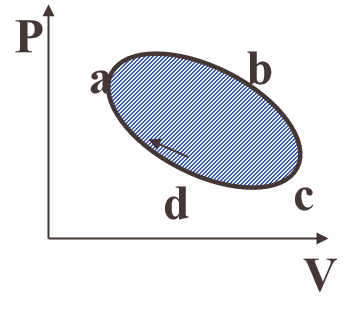
\includegraphics[width=0.2\linewidth]{screenshot004}
		\caption{}
		\label{fig:screenshot004}
	\end{figure}
	这样的图像,如果过程是顺时针的,我们就称之为正循环(表明气体对外界做正功),如果是逆时针的,我们就称为逆循环(表明气体对外界做负功)。接下来我们就要对其的循环进行仔细研究。
	
	我们知道,在正循环中,adbc所围成的面积就是表示其对外的做功量$A$,又由于其在循环结束之后内能不变,故其在循环过程吸收的热量$Q_{1}$必然要大于放出的热量$Q_{2}$(因为还有要对外界做功),并且有$Q_{1}-Q_{2}=A$。在这样一个循环里,气体从某些高温热源吸热,然后对外界进行做功,对这样一个“热变功”的循环,我们常常像研究其的效率,顾名思义,就是输入多少热,会做多少功,定义如下
	
	\begin{definition}[热机效率]
		我们称在一次循环过程中,工作物质对外做的净功与它从高温热源吸收的热量之比为热机效率。数学表达式如下
		\begin{equation*}
			\eta=\frac{A}{Q_{\text{吸}}}=\frac{Q_{\text{吸}}-Q_{\text{放}}}{Q_{\text{吸}}}=1-\frac{Q_{\text{放}}}{Q_{\text{吸}}}
		\end{equation*}
		用图像来表示能量的流动就如下,$W$为其对外界所做的功。
	\end{definition}
		\begin{figure}[h]
		\centering
		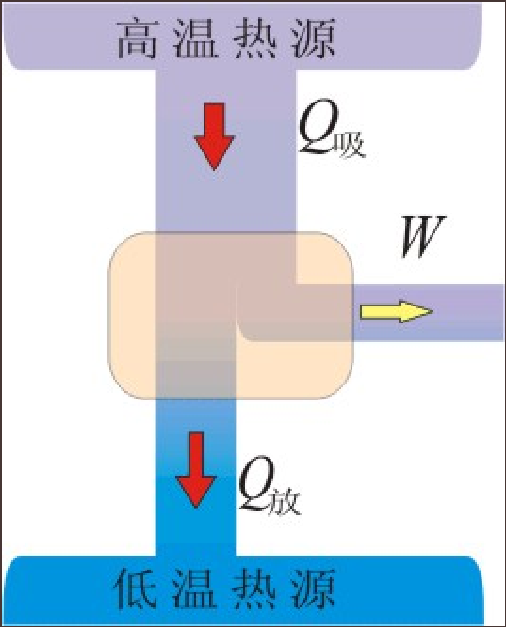
\includegraphics[width=0.2\linewidth]{screenshot006}
		\caption{}
		\label{fig:screenshot006}
	\end{figure}
	同样的,我们来研究以下逆循环,在逆循环的过程中,其的图像面积表示系统对外界做的负功的数值$A$,由热力学第一定律,就有系统放出的热量$Q_{\text{放}}$的数值是大于$Q_{\text{吸}}$的,且有$Q_{\text{放}}-Q_{\text{吸}} =A$,在这样一个循环里,气体从低温热源吸热,向高温热源放热,显然是不可能自发进行的,因此需要外界对其做功才能进行,这就是我们生活中的制冷机,对此,其的制冷效率便是我们关心的,即我们给它多少功,它能够吸多少热,定义如下
	\begin{definition}[制冷效率]
		我们称在一次循环中,制冷机从低温热源吸取的热量与外界做功之比为制冷效率。
		数学表达式如下
		\begin{equation*}
			\varepsilon =\frac{Q_{\text{吸}}}{A}=\frac{Q_{\text{吸}}}{Q_{\text{放}}-Q_{\text{吸}}}
		\end{equation*}
		用图像表示能量的流动,就如下,其中$W$为外界对系统做的功
	\end{definition}
	\begin{figure}[H]
		\centering
		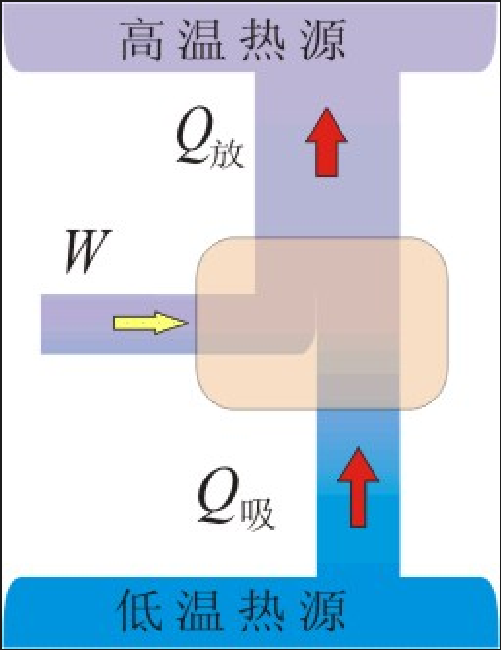
\includegraphics[width=0.2\linewidth]{screenshot009}
		\caption{}
		\label{fig:screenshot009}
	\end{figure}
	
	在了解循环的定义之后,我们就要来到其在生活中的应用,其中最著名的莫过于卡诺循环,定义如下
	\begin{definition}[卡诺循环]
		工作物质只与两个恒定热源(一个高温热源,一个低温热源)交换热量。整个循环过程是由两个绝热过程和两个等温过程构成,这样的循环过程称为卡诺循环。
	\end{definition}
	其循环图如下
	\begin{figure}[H]
		\centering
		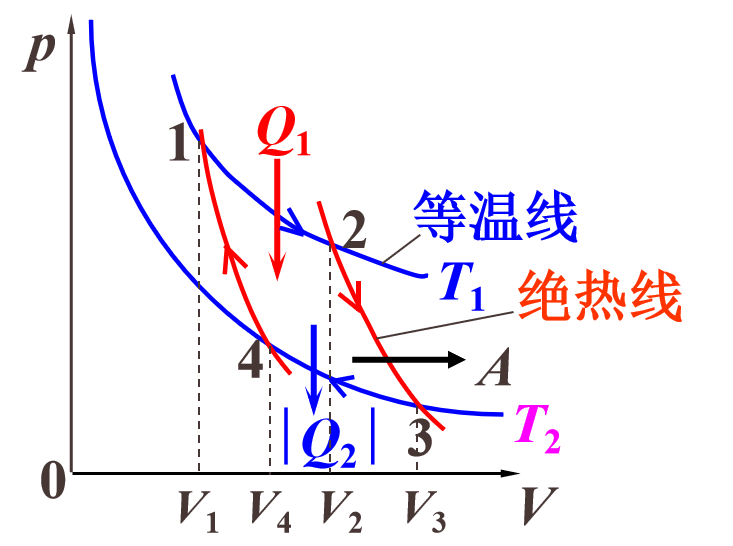
\includegraphics[width=0.4\linewidth]{screenshot010}
		\caption{}
		\label{fig:screenshot010}
	\end{figure}
	1到2是等温过程,系统体积变大,气体对外界做正功,就有
	\begin{equation*}
		W_{1\rightarrow 2}=\nu RT\ln\mathrm{(}\frac{V_2}{V_1})
	\end{equation*}
	此时气体要从高温热源吸热。
	
	2到3是绝热过程,不参与吸放热,对气体列绝热方程,有
	\begin{equation*}
		\frac{V_{2}^{\gamma-1}}{T_{1}}=\frac{V_{3}^{\gamma-1}}{T_{2}}
	\end{equation*}
	
	3到4是等温过程,系统体积变小,气体对外界做负功,就有
	\begin{equation*}
		W_{3\rightarrow 4}=\nu RT\ln\mathrm{(}\frac{V_4}{V_3})
	\end{equation*}
	此时气体要向低温热源放热
	
	4到1是绝热过程,对气体列绝热方程,有
	\begin{equation*}
		\frac{V_{1}^{\gamma-1}}{T_{1}}=\frac{V_{4}^{\gamma-1}}{T_{2}}
	\end{equation*}
	
	以上就是对卡诺循环过程的分析。其能量流向图如下
	\begin{figure}[H]
		\centering
		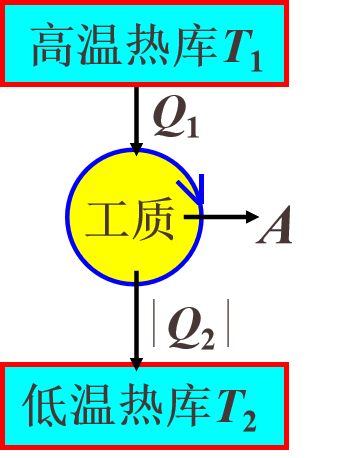
\includegraphics[width=0.3\linewidth]{screenshot011}
		\caption{}
		\label{fig:screenshot011}
	\end{figure}
	
	我们可以得到其热机循环的效率
	\begin{equation*}
		\eta=\frac{A}{Q_{\text{吸}}}=\frac{Q_{\text{吸}}-Q_{\text{放}}}{Q_{\text{吸}}}=1-\frac{Q_{\text{放}}}{Q_{\text{吸}}}=1-\frac{T_{2}}{T_{1}}
	\end{equation*}
	我们也可以得到其逆循环的能量流向图
	\begin{figure}[H]
		\centering
		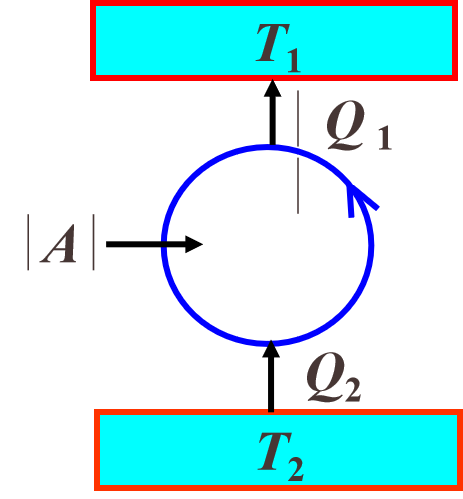
\includegraphics[width=0.3\linewidth]{screenshot012}
		\caption{}
		\label{fig:screenshot012}
	\end{figure}
	同理我们也可以得到其制冷系数
	\begin{equation*}
		\varepsilon =\frac{Q_{\text{吸}}}{A}=\frac{Q_{\text{吸}}}{Q_{\text{放}}-Q_{\text{吸}}}=\frac{T_{2}}{T_{1}-T_{2}}
	\end{equation*}
	这个就是重要的卡诺循环。为啥重要呢,你会发现,卡诺循环的热机和制冷机的效率仅与其热源温度有关,与其介质无关。这就是著名的卡诺定理
	\begin{theorem}[卡诺定理]
		工作在相同温度的高、低温热库之间的一切可逆机的效率都相等,与工作物质无关
	\end{theorem}
	
	有了这个定理,我们就可以得到一个有趣的结论
	\begin{conclusion}
		\begin{equation*}
			\left( \frac{\partial U}{\partial V} \right) _T=T\left( \frac{\partial p}{\partial T} \right) _V-p
		\end{equation*}
		这个结论,找到了内能,压强,温度,体积这些气体的状态参量之间的关系
	\end{conclusion}

	\section{热一+物态方程习题}
	\begin{example}
		分别通过下列过程把标准状态下的0.014 kg氮气压缩为原体积的一半
		
		(1)等温过程
		
		(2)绝热过程
		
		(3)等压过程
		
		试分别求出在这些过程中气体内能的改变,传递的热量和对外界气体所做的功,记其$C_{V,m}=\frac{5}{2}R$
	\end{example}
	\begin{solution}
		(1)由等温过程,温度不变,内能不变,其做功满足以下式子
		\begin{equation*}
			W=-\nu RT\ln\mathrm{(}\frac{V_2}{V_1})=-Q
		\end{equation*}
		代入数据,解得
		\begin{equation*}
			W=786J,Q=-786J
		\end{equation*}
		表明气体对外界做负功,放热
		
		(2)绝热过程,满足以下公式
		\begin{equation*}
			\frac{V_{1}^{\gamma-1}}{T_{1}}=\frac{V_{2}^{\gamma-1}}{T_{2}}
		\end{equation*}
		又因为气体与外界热交换数值为0,故其体内能的改变量与气体和外界做的功一样
		满足
		\begin{equation*}
			W=U=\nu C_{V,m}\varDelta T
		\end{equation*}
		代入上述绝热方程,有
		\begin{equation}
			W=U=\nu C_{V,m}T_1((\frac{V_1}{V_2})^{\gamma -1}-1)
		\end{equation}
		代入数据,解得
		\begin{equation*}
			W=U=906J
		\end{equation*}
		此时气体对外界做负功,气体内能增加
		
		(3)等压过程,有
		\begin{equation*}
			\frac{V_{1}}{T_{1}}=\frac{V_{2}}{T_{2}}
		\end{equation*}
		内能改变量满足
		\begin{equation*}
			U=\nu C_{V,m}\varDelta T
		\end{equation*}
		代入可得
		\begin{equation*}
			U=\nu C_{V,m}\varDelta T=\nu C_{V,m}T_1((\frac{V_1}{V_2})-1)
		\end{equation*}
		在等压过程中,气体与外界的热交换量$Q$满足
		\begin{equation*}
			Q=\nu C_{p,m}\varDelta T
		\end{equation*}
		代入公式,解得
		\begin{equation*}
			U=-1.42\times10^{3}J,Q=-1.98\times10^{3}J
		\end{equation*}
		此时内能减少,气体放热
		
		由热力学第一定律,有
		\begin{equation*}
			U=W+Q
		\end{equation*}
		解得
		\begin{equation*}
			W=5.76\times10^{3}J 
		\end{equation*}
		此时气体对外界做负功
	\end{solution}
	
	\begin{example}
		室温下一定量理想气体氧的体积为2.3L,压强为$1.01$$\times$$10^{5}$  Pa,经过一多方过程后体积变为4.1L,压强变为原来的一半,试求
		
		(1)多方指数n
		
		(2)内能的变化
		
		(3)吸收的热量
		
		(4)膨胀时气体对外界做的功,
		记其$C_{V,m}=\frac{5}{2}R$
	\end{example}
	\begin{solution}
		(1)对于多方过程,我们有
		\begin{equation*}
			p_1V_{1}^{n}=p_2V_{2}^{n}
		\end{equation*}
		代入数据,解得
		\begin{equation*}
			n=1.2
		\end{equation*}
		
		(2)对于任意过程的内能变化,我们有
		\begin{equation*}
			U=\nu C_{V,m}\varDelta T
		\end{equation*}
		又因为题目给的数据是压强,有理想气体状态方程可得
		\begin{equation*}
			pV=\nu RT
		\end{equation*}
		代入上式,有
		\begin{equation*}
			U=\frac{5}{2}(p_{2}V_{2}-p_{1}V_{1}) 
		\end{equation*}
		代入数据,有
		\begin{equation*}
			U=-63J
		\end{equation*}
		
		(3)对于多方过程的吸放热,我们有
		\begin{equation*}
			Q=\nu c\varDelta T
		\end{equation*}
		又因为多方过程的热容满足以下关系
		\begin{equation*}
			C=C_{V,m}-\frac{R}{n-1}
		\end{equation*}
		代入上式,可解得
		\begin{equation*}
			Q=63J
		\end{equation*}
		
		(4)由热力学第一定律,有
		\begin{equation*}
			U=W+Q
		\end{equation*}
		代入数据,解得
		\begin{equation*}
			W=-126J
		\end{equation*}
		即气体对外做功$126J$
	\end{solution}
	\begin{example}
		0.008kg氧气,原来温度为27℃,体积为0.41L,若
		
		(1)经过绝热膨胀体积增为4.1L
		
		(2)先经过等温过程再经过等体过程达到(1)同样的状态
		
		试分别计算在以上两种过程中外界对气体所做的功,记氧气的$C_{V,m}=\frac{5}{2}R$
	\end{example}
	\begin{solution}
		(1)对于绝热过程气体对外界做的功$W$,满足
		\begin{equation*}
			W=\frac{p_1V_1}{\gamma -1}((\frac{V_1}{V_2})^{\gamma -1}-1)
		\end{equation*}
		代入数据,解得
		\begin{equation*}
			W=-9.38\times10^{3}J
		\end{equation*}
		
		(2)对于等温过程,气体对外界做的功满足
		\begin{equation*}
			W_{1}=\nu RT\ln\mathrm{(}\frac{V_2}{V_1})
		\end{equation*}
		代入数据,解得
		\begin{equation*}
				W_{1}=-1.44\times10^{4}J
		\end{equation*}
		对于等容过程,气体不对外界做功,因此整个过程气体对外界做的功为等温过程所做的功
	\end{solution}
	
	\begin{example}
		在标准状态下,1 mol的双原子气体先经过一绝热过程,再经过一等温过程,最后压强和体积均增为原来的两倍,求整个过程中系统吸收的热量。若先经过等温过程,再经过绝热过程而达到同样的状态,则结果是否相同?
	\end{example}
	\begin{solution}
		先绝热后等温
		
		对于绝热过程,气体不与外界进行热量交换,与是此时$Q_{1}=0$
		对此时列绝热方程,有
			\begin{equation*}
			p_{1}V_{1}^{\gamma}=	p_{2}V_{2}^{\gamma},\frac{V_{1}^{\gamma-1}}{T_{1}}=\frac{V_{2}^{\gamma-1}}{T_{2}}
			\end{equation*}
		对于等温过程,我们有
		\begin{equation*}
			p_{2}V_{2}=p_{3}V_{3}
		\end{equation*}
		又有
		\begin{equation*}
			pV=\nu RT
		\end{equation*}
		解得
		\begin{equation*}
			T_{2}=4T_{1},V_{2}=\frac{1}{8}V_{1}
		\end{equation*}
		此时气体内能不变,吸收的热量数值由气体对外界所做的功决定,于是就有
		\begin{equation*}
			Q=-W=\nu RT_{1}\ln\mathrm{(}\frac{V_3}{V_2})
		\end{equation*}
		代入数据,解得
		\begin{equation*}
			Q=2.52\times10^{4}J
		\end{equation*}
		
		先等温再绝热
		
		对于等温过程,我们有
		\begin{equation*}
			p_{1}V_{1}=p_{2}V_{2}
		\end{equation*}
		又有
		\begin{equation*}
			pV=\nu RT
		\end{equation*}
		此时气体内能不变,吸收的热量数值由气体对外界所做的功决定,于是就有
		\begin{equation*}
			Q=-W=\nu RT_{1}\ln\mathrm{(}\frac{V_2}{V_1})
		\end{equation*}
		
		对于绝热过程,气体不与外界进行热量交换,与是此时$Q_{2}=0$
		对此时列绝热方程,有
		\begin{equation*}
			p_{2}V_{2}^{\gamma}=	p_{3}V_{3}^{\gamma},\frac{V_{2}^{\gamma-1}}{T_{2}}=\frac{V_{3}^{\gamma-1}}{T_{3}}
		\end{equation*}
		代入,解得
		\begin{equation*}
			V_{2}=16V_{1}
		\end{equation*}
		再代入前面的公式进行计算,有
		\begin{equation*}
			Q=6.3\times10^{4}J
		\end{equation*}
	\end{solution}
	~\\
	~\\
	
	\begin{example}
		如图所示,瓶内装有气体,一横截面为$A$的玻璃管通过瓶塞插入瓶内,玻璃管内放有一个质量为$m$光滑金属小球(像一个活塞)。设小球再、在平衡位置时,气体的体积为$V$,压强为$p=p_{0}+\frac{mg}{A}$($p_{0}$为大气压强)。再将小球稍向下移,然后放手,则小球将以周期为$T$在平衡位置附近做简谐运动,假定小球上下运动的过程中,瓶内气体运动的过程可以看作准静态过程
		证明
		
		(1)使小球进行简谐运动的准弹性力为
		\begin{equation*}
			F=-\frac{\gamma p A^{2}}{V}y
		\end{equation*}
		这里$	\gamma=\frac{	C_{p,m}}{ C_{V,m}}$,$y$为位移
		
		(2)小球进行简谐运动的周期为
		\begin{equation*}
			T=2\pi\sqrt{\frac{mV}{\gamma p A^{2}}}
		\end{equation*}
		
		(3)由此说明怎么测量$\gamma$
		
	\end{example}
	\begin{figure}[H]
		\centering
		\includegraphics[width=0.16\linewidth]{D:/MobileFile/qq_pic_merged_1684041998382}
		\caption{}
		\label{fig:qqpicmerged1684041998382}
	\end{figure}
	\begin{solution}
		(1)由于是绝热过程,满足以下关系
		\begin{equation*}
			pV^{\gamma}=\text{常数}
		\end{equation*}
		我们对等式进行求导,有
		\begin{equation*}
			V^{\gamma}dp=-\gamma pV^{\gamma-1}dV
		\end{equation*}
		我们将左右两边同时除以$V^{\gamma} $,可得到
		\begin{equation*}
			dp=-\frac{\gamma p}{V}dV
		\end{equation*}
		我们观察以下目前我们的式子和题目所给式子的差异,差别在于$A^{2}$和$y$
		
		考虑到
		\begin{equation*}
			F=dps
		\end{equation*}
		就有
		\begin{equation*}
		F=Adp=-A\frac{\gamma p}{V}dV
		\end{equation*}
		又因为
		\begin{equation}
			dV=Ay
		\end{equation}
		代入原式,有
		\begin{equation*}
			F=-\frac{\gamma p A^{2}}{V}y
		\end{equation*}
		~\\
		~\\
		
		(2)由于小球的简谐运动方程为
		\begin{equation*}
			m\overset{..}{y}+\frac{\gamma p A^{2}}{V}y=0
		\end{equation*}
		由此可得
		\begin{equation*}
			\omega =\sqrt{\frac{\gamma p A^{2}}{V}}
		\end{equation*}
		于是乎,振动周期$T$就为
		\begin{equation*}
			T=\frac{2\pi}{\omega}=2\pi\sqrt{\frac{mV}{\gamma p A^{2}}}
		\end{equation*}
		
		(3)化简周期,有
		\begin{equation*}
			\gamma =\frac{4\pi ^2mV}{A^2pT^2}
		\end{equation*}
		只需要测量这些数值即可
	\end{solution}
	
	\begin{example}
		仍如前提装置,设实验开始时,维持小球所在位置正好使瓶内气体压强仍为大气压强$p_{0}$,然后让小球在其重力作用下下落,下落一段距离$L$后又开始上升
		
		(1)证明:在这过程中小球克服准弹性力所做的功为
		\begin{equation*}
			\frac{\gamma p_{0}A^{2}L^{2}}{2V}
		\end{equation*}
		
		(2)上述的功由小球重力势能转化而来,试证明
		\begin{equation*}
			\gamma=\frac{2mgV}{p_{0}A^{2}L}
		\end{equation*}
		
		
	\end{example}
	\begin{solution}
		(1)我们不妨假设小球此时下降了很小的距离$y$
		由于是绝热过程,满足以下关系
		\begin{equation*}
			p_{0}V^{\gamma}=p_{1}(V-Ay)^{\gamma}
		\end{equation*}
		左右两边同除$(V-Ay)^{\gamma}$,有
		\begin{equation*}
			p_1=p_0\left( \frac{V}{V-yA} \right) ^{\gamma}=p_0\left( 1+\frac{yA}{V-yA} \right) ^{\gamma}
		\end{equation*}
		又因为$y$很小,于是就有下列近似计算
			\begin{equation*}
			p_1=p_0\left( \frac{V}{V-yA} \right) ^{\gamma}=p_0\left( 1+\frac{yA}{V-yA} \right) ^{\gamma}=p_0\left( 1+\frac{yA}{V} \right) ^{\gamma}
		\end{equation*}
		这里的话,答案用了一个很迷的近似计算,即
		\begin{equation*}
			(1+x)^{n}\approx1+nx
		\end{equation*}
		于是乎,就有
		\begin{equation*}
			p_1=p_0\left( \frac{V}{V-yA} \right) ^{\gamma}=p_0\left( 1+\frac{yA}{V-yA} \right) ^{\gamma}=p_0\left( 1+\frac{yA}{V} \right) ^{\gamma}=p_0\left( 1+\frac{\gamma yA}{V} \right) 
		\end{equation*}
		由此,下落很小一段距离,系统(小球+外界)对瓶内气体所做的功$W$为
		\begin{equation*}
			W=\int\limits_0^L{p_{1}Ady}
		\end{equation*}
		则小球压缩气体所做的功A为
		\begin{equation*}
			A=W-\int\limits_0^L{p_{0}Ady}=	\frac{\gamma p_{0}A^{2}L^{2}}{2V}
		\end{equation*}
		~\\
		~\\
		~\\
		当然,我们还有一种解法,由上一题,我们知道小球所受的弹性力大小为
		\begin{equation*}
			F=-\frac{\gamma p A^{2}}{V}y
		\end{equation*}
		对这一过程,有
		\begin{equation*}
			W=\int\limits_0^L{Fdy}=\int\limits_0^L{-\frac{\gamma p A^{2}}{V}ydy}=-\frac{\gamma p_{0}A^{2}L^{2}}{2V}
		\end{equation*}
		负号表明做气体对小球做负功。
		
		(2)对小球,由能量守恒,有
		\begin{equation*}
			mgL=\frac{\gamma p_{0}A^{2}L^{2}}{2V}
		\end{equation*}
		解得
		\begin{equation*}
			\gamma=\frac{2mgV}{p_{0}A^{2}L}
		\end{equation*}
	\end{solution}
	\begin{example}
		如图所示,用绝热壁做成一圆柱形的仪器。在容器中间放置一无摩擦的、绝热的可动活塞。活塞两侧各有n mol 的理想气体,开始状态均为$p_{0}$、$V_{0}$、$T_{0}$,设气体摩尔定容热容为常量,$\gamma=1.5$
		
		将一通电线圈放到活塞左侧气体中,对气体缓慢地加热,左侧气体膨胀的同时通过活塞压缩右侧气体,最后使右方气体压强增为$\frac{27}{8}p_{0}$,求
		
		(1)对活塞右侧气体做了多少功?
		
		(2)右侧气体的终温为?
		
		(3)左侧气体的终温为?
		
		(4)左侧气体吸收了多少热量?
	\end{example}
	\begin{figure}[H]
		\centering
		\includegraphics[width=0.2\linewidth]{D:/MobileFile/qq_pic_merged_1684042094342}
		\caption{}
		\label{fig:qqpicmerged1684042094342}
	\end{figure}
	\begin{solution}
		
		(1)根据题设信息,该过程为绝热过程,设其对右侧气体做的功为$W$,则有
		\begin{equation*}
			W=\frac{p_0V_0}{\gamma -1}((\frac{V_0}{V_1})^{\gamma -1}-1)
		\end{equation*}
		对右侧气体,绝热过程,有
		\begin{equation*}
				p_{0}V_{0}^{\gamma}=p_{1}V_{1}^{\gamma}
		\end{equation*}
		代入,解得
		\begin{equation*}
			W=p_{0}V_{0}
		\end{equation*}
		此时外界对气体做正功
		
		(2)对右侧气体,由绝热过程,有
		\begin{equation*}
			\frac{T_{0}^{\gamma}}{p_{0}^{\gamma -1}}=\frac{T_{1}^{\gamma}}{p_{1}^{\gamma -1}}
		\end{equation*}
		代入数据,解得
		\begin{equation*}
			T_{1}=\frac{3}{2}T_{0}
		\end{equation*}
		
		(3)对左侧气体分析,我们知道,如果左右两边压强不等,那么活塞不会达到平衡
		于是乎,左右两边压强相等。并且左右两边的体积满足
		\begin{equation*}
			V_{\text{左}}+V_{\text{右}}=2V_{0}
		\end{equation*}
		对右侧气体,由绝热方程,有
		\begin{equation*}
			p_{0}V_{0}^{\gamma}=p_{1}V_{\text{右}}^{\gamma}
		\end{equation*}
		代入数据,可计算出
		\begin{equation*}
			V_{\text{右}}=\frac{4}{9}V_{0}
		\end{equation*}
		再代入上式,可计算出
		\begin{equation*}
				V_{\text{左}}=\frac{14}{9}V_{0}
		\end{equation*}
		对左边的气体,由理想气体状态方程,有
		\begin{equation*}
			\frac{p_1V_{\text{左}}}{T_2}=\frac{p_0V_0}{T_0}
		\end{equation*}
		解得
		\begin{equation*}
			T_{2}=\frac{21}{4}T_{0}
		\end{equation*}
		
		(4)求内能,吸放热,做功之间的关系,闭着眼睛写热一
		\begin{equation*}
			\varDelta U=A+Q
		\end{equation*}
		外界对气体做的功我们已经知道,此时我们只需要求$\varDelta U$即可,其满足
		\begin{equation}
			\varDelta U=\nu C_{V,m}\varDelta T
		\end{equation}
		此时我们并不知道定容摩尔热容的数值,但我们知道
		\begin{equation*}
			\frac{C_{V,m}}{C_{p,m}}=\gamma,C_{V,m}+R=C_{p,m}
		\end{equation*}
		代入上式,我们可得
		\begin{equation*}
			\varDelta U=\frac{17}{2}nRT_{0}
		\end{equation*}
		又因为左边气体对右边气体做正功,于是右边气体对左边气体做负功,就有
		\begin{equation*}
			Q=\frac{17}{2}nRT_{0}+p_{0}V_{0}
		\end{equation*}
		又因为
		\begin{equation*}
			pV=\nu RT
		\end{equation*}
		代入可得
		\begin{equation*}
				Q=\frac{19}{2}nRT_{0}
		\end{equation*}
	\end{solution}
	\section{焓的计算}
	\begin{example}
		设1mol的固体的物态方程可写作
		\begin{equation*}
			V_{m}=V_{m0}+aT+bp
		\end{equation*}
		内能可表示为
		\begin{equation*}
			U_{m}=cT-apT
		\end{equation*}
		其中,$a$、$b$、$c$和$V_{m0}$为常量,试求
		
		(1)摩尔焓的表达式
		
		(2)摩尔热容$C_{V,m},C_{p,m}$
	\end{example}
	\begin{solution}
		
		(1)由焓的定义
		\begin{equation*}
			H=U+pV
		\end{equation*}
		代入数据可算得
		\begin{equation*}
			H=cT+pV_{m_{0}}+bp^{2}
		\end{equation*}
		
		(2)由定压摩尔热容的定义,有
		\begin{equation*}
				C_{p}=\lim_{\varDelta T\rightarrow 0} \frac{	\left( \varDelta Q \right) _p}{\varDelta T}=\left( \frac{\partial H}{\partial T} \right) _p
		\end{equation*}
		就是把$p$看成常数,让$H$对$T$求导,于是就有
		\begin{equation*}
			C_{p,m}=c
		\end{equation*}
		
		我们再看定容摩尔热容的定义,有
		\begin{equation*}
				C_{V}=\lim_{\varDelta T\rightarrow 0} \frac{	\left( \varDelta Q \right) _V}{\varDelta T}=\left( \frac{\partial U}{\partial T} \right) _V
		\end{equation*}
		又因为
		\begin{equation*}
			U_{m}=cT-apT
		\end{equation*}
		于是就有
		\begin{equation*}
			C_{V,m}=c-a\left[ \frac{\partial \left( pT \right)}{\partial T} \right] _V
		\end{equation*}
		由乘法求导数的链式法则,有
		\begin{equation*}
			\left[ \frac{\partial \left( pT \right)}{\partial T} \right] _V=p+T(\frac{\partial p}{\partial T})_{V}
		\end{equation*}
		代入原式,有
		\begin{equation*}
			C_{V,m}=c-ap-aT(\frac{\partial p}{\partial T})_{V}
		\end{equation*}
		现在我们要求$(\frac{\partial p}{\partial T})_{V}$,观察到
		\begin{equation*}
			V_{m}=V_{m0}+aT+bp
		\end{equation*}
		于是就有
		\begin{equation*}
			(\frac{\partial p}{\partial T})_{V}=-\frac{a}{b}
		\end{equation*}
		代入前式,有
		\begin{equation*}
			C_{V,m}=c-ap-\frac{a^{2}T}{b}
		\end{equation*}
		代换掉$p$,有
		\begin{equation*}
				C_{V,m}=c-\frac{a}{b}(V_{m}-V_{m_{0}})+\frac{2a^{2}T}{b}
		\end{equation*}
	\end{solution}
	~\\
	\section{循环过程习题}
	
	\begin{example}
		如图所示,为一个理想气体($\gamma$已知)的循环过程,其中$CA$为绝热过程。$A$点的状态参量($T,V_{1}$)和$B$点的状态参量($T,V_{2}$)均为已知
		
		(1)气体在$A$到$B$,$B$到$C$两过程中各和外界交换热量吗?是放热还是吸热?
		
		(2)求$C$点的状态参量
		
		(3)这个循环是不是卡诺循环?
		
		(4)求这个循环的效率
	\end{example}
	\begin{figure}[H]
		\centering
		\includegraphics[width=0.2\linewidth]{D:/MobileFile/qq_pic_merged_1684042081374}
		\caption{}
		\label{fig:qqpicmerged1684042081374}
	\end{figure}
	\begin{solution}
		
		(1)A到B是等温过程,气体从外界吸热
		B到C是等体过程,气体放热
		
		(2)CA为绝热过程,由绝热方程,有
		\begin{equation*}
			T_C\left( V_2 \right) ^{\gamma -1}=T_1\left( V_1 \right) ^{\gamma -1}
		\end{equation*}
		解得
		\begin{equation*}
			T_{C}=T(\frac{V_{1}}{V_{2}})^{\gamma-1}
		\end{equation*}
		
		(3)卡诺循环是由两个绝热过程加上两个等温过程,显然这个不是
		
		(4)B到A等温过程,外界对气体做功,气体吸热,有
		\begin{equation*}
			W_{B\rightarrow A}=-\nu RT\ln\mathrm{(}\frac{V_2}{V_1})=-Q_{1}
		\end{equation*}
		
		B到C等体过程,气体放热,有
		\begin{equation*}
			Q_{2}=\varDelta U=\nu C_{V,m}(T-T_{C})=\nu \frac{R}{\gamma-1}[T-(T(\frac{V_{1}}{V_{2}})^{\gamma-1})]
		\end{equation*}
		又因为
		\begin{equation*}
			\eta=1-\frac{Q_{\text{放}}}{Q_{\text{吸}}}
		\end{equation*}
		代入可得
		\begin{equation*}
			\eta=1-\frac{ \frac{R}{\gamma-1}[T-(T(\frac{V_{1}}{V_{2}})^{\gamma-1})]}{ RT\ln\mathrm{(}\frac{V_2}{V_1})}=1-\dfrac{1-(\frac{V_{1}}{V_{2}})^{\gamma-1}}{(\gamma-1)\ln\mathrm{(}\frac{V_2}{V_1})}
		\end{equation*}
	\end{solution}
	
	\begin{example}
		设一动力装置由一个热机和一个制冷机组合而成。热机靠燃料燃烧时放出的热量工作,同时向暖气系统的水放热,并带动制冷机。制冷机自天然蓄水池中吸热,也向暖气系统放热。设热机锅炉的温度为$t_{1}$=210℃,天然水的温度为$t_{2}$=15℃,暖气系统的温度为$t_{3}$=60℃,燃料的燃烧热5000 kcal$\cdot$kg$^{-1}$,试求燃烧1.00kg燃料,暖气系统所得的热量。假设热机和制冷机的工作循环都是理想卡诺循环。	
	\end{example}
	\begin{solution}
		本题的循环能量流向图如下
		\begin{figure}[H]
			\centering
			\includegraphics[width=0.2\linewidth]{D:/MobileFile/qq_pic_merged_1684236092854}
			\caption{}
			\label{fig:qqpicmerged1684236092854}
		\end{figure}
		其中Ⅰ为热机,Ⅱ为制冷机,$Q_{3}+Q_{4}$即为我们要求出的暖气系统所得的热量,又因为$Q_{3}=Q_{1}-A,Q_{4}=A+Q_{2}$,我们实际要求出的,是$Q_{1}+Q_{2}$
		
		
		首先我们要求出热机传输给制冷机的能量$A$,由于卡诺机的效率仅和两个热源的温度有关,则有
		\begin{equation*}
			\eta=1-\frac{T_{3}}{T_{1}}	
		\end{equation*}
		则我们可以算出$A$的数值
		\begin{equation*}
			A=\eta Q_{1}=(1-\frac{T_{3}}{T_{1}})	Q_{1}
		\end{equation*}
		然后我们可以凭此来算出$Q_{2}$
		
		由于卡诺机的效率仅和两个热源的温度有关,我们可以算出
		\begin{equation*}
			\varepsilon=\frac{Q_{2}}{A}=\frac{T_{2}}{T_{3}-T_{2}}
		\end{equation*}
		解得
		\begin{equation*}
			Q_{2}=\frac{T_{2}}{T_{3}-T_{2}}A
		\end{equation*}
		当燃烧1kg燃料时,我们代入数据,可得
		\begin{equation*}
			Q_{1}+Q_{2}=1.492\times10^{4}kcal
		\end{equation*}
	\end{solution}	
	
	\begin{example}
		一理想气体准静态卡诺循环,当热源温度为100℃,冷却器温度为0℃时,净做功800J.今维持冷却器温度不变,提高热源温度,使净做功增加为1600J,则这时
		
		(1)热源的温度为多少?
		
		(2)效率增大到多少?
		(设这两个循环都工作于相同的两绝热线之间。)
	\end{example}
	\begin{solution}
		
		(1)由于处于相同绝热线之间,又低温热源温度不变,所以其吸收的热量$Q_{2}$都一样
		于是有
		\begin{equation*}
			Q_{2}=A_{1}\frac{T_{2}}{T_{1}-T_{2}}=A_{2}\frac{T_{2}}{T'_{1}-T_{2}}
		\end{equation*}
		代入数据,解得
		\begin{equation*}
			T'_{1}=473K
		\end{equation*}
		
		(2)由于卡诺机的效率仅和热源有关,故
		\begin{equation*}
			\eta=1-\frac{T_{2}}{T'_{1}}=42.3 \%
		\end{equation*}
	\end{solution}
	\begin{example}
		一可逆卡诺机低温热源的温度为7.0℃,效率为40$\%$.若要将其效率提高到50$\%$,则高温热源的温度需要提高几摄氏度?
	\end{example}
	\begin{solution}
	由于卡诺机的效率仅和热源有关,故
	\begin{equation*}
			\eta=1-\frac{T_{2}}{T_{1}}=40 \%
	\end{equation*}	
	代入数据,解得
	\begin{equation*}
		T_{1}=476K
	\end{equation*}
	当效率为50$\%$时,我们有
		\begin{equation*}
		\eta=1-\frac{T_{2}}{T_{3}}=50 \%
	\end{equation*}	
	代入数据,解得
	\begin{equation*}
		T_{3}=560K
	\end{equation*}
	于是,我们要增加的温度为560-476=93摄氏度
	\end{solution}
	\section{那个抽象公式的应用——了解即可}
	\begin{example}
		(1)证明,对1mol范德瓦尔斯气体,有
		\begin{equation*}
			\left( \frac{\partial U_m}{\partial V_m} \right) _T=\frac{a}{V_{m}^{2}}
		\end{equation*}
		
		(2)由(1)证明
		\begin{equation*}
			U_m=U_{m_0}+\int_{T_0}^T{C_{V,m}dT}+a\left( \frac{1}{V_{m_0}}-\frac{1}{V_m} \right) 
		\end{equation*}
		
		(3)设$C_{V,m}$为常量,证明上式可写为
		\begin{equation*}
			U_m=U\prime_{m_0}+C_{V,m}T+\frac{a}{V_m}
		\end{equation*}
		其中$U\prime_{m_0}=U_{m_0}-C_{V,m}T_{0}+\frac{a}{V_{m_{0}}}$
	\end{example}
	\begin{solution}
		
		(1)对于范德瓦尔斯气体,我们有
		\begin{equation}
			p=\frac{RT}{V_m-b}-\frac{a}{V_{m}^{2}}
		\end{equation}
		对于该气体,我们有
		\begin{equation}
			\left( \frac{\partial U_{m}}{\partial V_{m}} \right) _T=T\left( \frac{\partial p}{\partial T} \right) _{V_{m}}-p
		\end{equation}
		于是我们要求$\left( \frac{\partial p}{\partial T} \right) _{V_{m}}$
		
		由(5.4),我们可以求得
		\begin{equation}
			\left( \frac{\partial p}{\partial T} \right) _{V_{m}}=\frac{R}{V_m-b}
		\end{equation}
		将(5.6),(5.4)代入(5.5),有
		\begin{equation*}
			\left( \frac{\partial U_m}{\partial V_m} \right) _T=\frac{a}{V_{m}^{2}}
		\end{equation*}
		
		(2)由于内能是关于温度和体积的函数,即$U(V,T)$
		则有
		\begin{equation}
			dU_m=\left( \frac{\partial U_m}{\partial V_m} \right) _TdV_m+\left( \frac{\partial U_m}{\partial T} \right) _{V_m}dT
		\end{equation}
		又因为
		\begin{equation}
			\left( \frac{\partial U_m}{\partial V_m} \right) _T=\frac{a}{V_{m}^{2}},\left( \frac{\partial U_m}{\partial T} \right) _{V_m}=C_{V,m}
		\end{equation}
		将其代入(5.7),有
		\begin{equation*}
			dU_m=\frac{a}{V_{m}^{2}}dV_m+C_{V,m}dT
		\end{equation*}
		对其积分,有
		\begin{equation*}
			\int\limits_{U_{m_0}}^{U_m}{}dU_m=\int\limits_{V_{m_0}}^{V_m}{}\frac{a}{V_{m}^{2}}dV_m+\int\limits_{T_0}^T{}C_{V,m}dT
		\end{equation*}
		计算得出
		\begin{equation*}
			U_m=U_{m_0}+\int_{T_0}^T{C_{V,m}dT}+a\left( \frac{1}{V_{m_0}}-\frac{1}{V_m} \right) 
		\end{equation*}
		
		(3)因为$C_{V,m}$为常数,有
		\begin{equation*}
				U_m=U_{m_0}+\int_{T_0}^T{C_{V,m}dT}+a\left( \frac{1}{V_{m_0}}-\frac{1}{V_m} \right)=U_{m_0}+C_{V,m}(T-T_{0})+a\left( \frac{1}{V_{m_0}}-\frac{1}{V_m} \right)
		\end{equation*}
		化简可得
		\begin{equation*}
			U_m=U\prime_{m_0}+C_{V,m}T+\frac{a}{V_m}
		\end{equation*}
		其中$U\prime_{m_0}=U_{m_0}-C_{V,m}T_{0}+\frac{a}{V_{m_{0}}}$
	\end{solution}
	 \begin{example}
	 	设有1 mol的范德瓦尔斯气体,证明其准静态绝热过程方程满足
	 	\begin{equation*}
	 		T\left( V_m-b \right) ^{\frac{R}{C_{V,m}}}=\text{常量}
	 	\end{equation*}
	 \end{example}
	 \begin{solution}
	 	对于范德瓦尔斯气体,我们有(上题的结论,我偷个懒)
	 	\begin{equation}
	 		dU_m=\frac{a}{V_{m}^{2}}dV_m+C_{V,m}dT
	 	\end{equation}
	 	由绝热过程,我们有
	 	\begin{equation*}
	 		\text{đ}Q=0,dU_{m}=\text{đ}A
	 	\end{equation*}
	 	又因为在准静态过程,我们有
	 	\begin{equation*}
	 		\text{đ}A=-pdV_{m}
	 	\end{equation*}
	 	对于范德瓦尔斯气体,我们有
	 	\begin{equation}
	 		p=\frac{RT}{V_m-b}-\frac{a}{V_{m}^{2}}
	 	\end{equation}
	 	于是式子化简为
	 	\begin{equation}
	 	\text{đ}A=-pdV_{m}=-(\frac{RT}{V_m-b}-\frac{a}{V_{m}^{2}})dV_{m}
	 	\end{equation}
	 	将(5.11)代入(5.9),有
	 	\begin{equation*}
	 		\frac{C_{V,m}}{T}dT=-\left( \frac{RT}{V_m-b}-\frac{a}{V_{m}^{2}} \right) dV_m
	 	\end{equation*}
	 	对其积分,可得
	 	\begin{equation*}
	 		\ln T=-\frac{R}{C_{V,m}}\ln(V_m-b)+\text{常量}
	 	\end{equation*}
	 	化简,有
	 	\begin{equation*}
	 		\ln T+\ln \left( V_m-b \right) ^{\frac{R}{C_{V,m}}}=\ln T\left( V_m-b \right) ^{\frac{R}{C_{V,m}}}
	 	\end{equation*}
	 	同取指数,有
	 	\begin{equation*}
	 		T\left( V_m-b \right) ^{\frac{R}{C_{V,m}}}=\text{常量}
	 	\end{equation*}
	 \end{solution}
	\chapter{热力学第二定律}
	\section{导学}
	这一章的话,重点知识不是很多,主要是热力学第二定律的两个表述,可逆与不可逆以及作为扩展知识的熵。
	\section{前置知识}
	在上一章节,热力学第一定律告诉我们:能量不可能凭空的产生和消失。这从理论上表明了第一类永动机(不需要供能就可对外界一直做功)是不可能成立的。既然这个方向不成立,那么我们可不可以发明一个第二类永动机,这类永动机满足热力学第一定律,但是其热机效率可以达到百分之百呢?生活中的经验告诉我们,这个显然是不成立的,为何?这就来到了本章第一个重点——热力学第二定律,对于其有两种表述
	\begin{theorem}[热力学第二定律]
		开氏表述:其唯一效果是热量全部转变为功的过程是不可能的
		
		克氏表述:热量不能自动地从低温物体传向高温物体
	\end{theorem}
	开氏表述就从理论上解释了第二类永动机不成立的原因。开氏表述与克氏表述本质上是相同的:都揭示了一切与热现象有关的实际宏观过程都不可逆,那么问题来了——何为可逆,何为不可逆呢?
	这就来到了我们第二个重点部分——可逆与不可逆过程
	\begin{definition}[可逆过程]
		每一步可在相反的方向进行而不引起外界的其他任何影响的过程为可逆过程
	\end{definition}
	\begin{definition}[不可逆过程]
		每一步都不可在相反的方向进行而不引起外界的其他任何影响的过程为不可逆过程
	\end{definition}
	\begin{note}
		(1)一切自发过程都是不可逆过程。
		
		(2)准静态过程(无限缓慢) +无摩擦的过程是可逆过程。
		
		(3)一切实际过程都是不可逆过程
		
		(4)不可逆过程不是不能逆向进行,而是说当过程逆向进行时,逆过程在外界留下的痕迹不能将原来正过程的痕迹完全消除
	\end{note}
	纯粹的理论判断,确乎让人有点摸不着头脑,那有没有什么数学上的表达式,能够更为直观地判断出一个过程是否可逆呢?为此,克劳修斯引入了熵的概念,这个概念又是如何引入的?这就是接下来我们要研究的
	
	我们先定义$Q_{rev}$为在可逆过程中系统吸收(放出)的热量
	
	然后考虑这样一个积分:
	\begin{equation*}
		\oint{\frac{\text{đ}Q_{rev}}{T}}=0
	\end{equation*}
	表明了积分
	\begin{equation*}
		\int\limits_A^B{\frac{\text{đ}Q_{rev}}{T}}
	\end{equation*}
	只和其初末态有关与其过程无关,因此,我们可以定义一个态函数,称之为熵$(S)$,定义如下
	\begin{equation*}
		dS=\frac{\text{đ}Q_{rev}}{T}
	\end{equation*}
	从而有
	\begin{equation*}
		S(B)-S(A)=\int\limits_A^B{\frac{\text{đ}Q_{rev}}{T}}
	\end{equation*}
	对于一个绝热过程,有
	\begin{equation*}
		\text{đ}Q_{rev}=0
	\end{equation*}
	因此绝热过程的熵不变,因而绝热过程是一个\textbf{等熵过程}。
	
	有了熵的定义之后,我们再此审视一下可逆与不可逆过程。
	由于熵是根据热量的可逆变化来定义的,由于$S$是态函数,所以$S$沿着封闭路径的积分为0,即
	\begin{equation*}
		\oint{\frac{\text{đ}Q_{rev}}{T}}=0
	\end{equation*}
	我们现在考虑这样一个回路,它包括一个不可逆部分a到b和一个可逆部分b到a
	\begin{figure}[H]
		\centering
		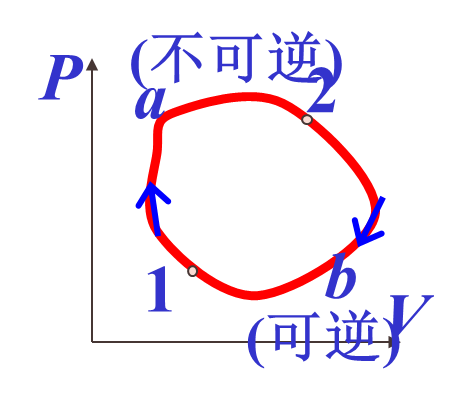
\includegraphics[width=0.2\linewidth]{screenshot013}
		\caption{}
		\label{fig:screenshot013}
	\end{figure}
	由克劳修斯不等式,有
	\begin{equation*}
		\oint{\frac{\text{đ}Q_{}}{T}}\le0
	\end{equation*}
	将左边详细地写出来,有
	\begin{equation*}
		\int\limits_a^b{\frac{\text{đ}Q_{}}{T}}+\int\limits_b^a{\frac{\text{đ}Q_{rev}}{T}}\le0
	\end{equation*}
	整理后,有
	\begin{equation*}
		\int\limits_a^b{\frac{\text{đ}Q_{}}{T}}\le\int\limits_a^b{\frac{\text{đ}Q_{rev}}{T}} 
	\end{equation*}
	无论a,b两状态多么接近,这个不等式依旧成立,故有
	\begin{equation*}
		dS=\frac{\text{đ}Q_{rev}}{T}\ge\frac{\text{đ}Q_{}}{T}
	\end{equation*}
	我们考虑一个热孤立系统,在这个系统中,有
	\begin{equation*}
		\text{đ}Q_{rev}=0
	\end{equation*}
	故上述不等式变为
	\begin{equation*}
		dS\ge 0
	\end{equation*}
	这就变成了一个特别重要的方程,这个方程事实上就是热力学第二定律的另一种表述,其表明了热孤立系统的任意变化的结果必是熵保持不变(可逆过程)或者熵变大(不可逆过程)这就给予了我们热力学第二定律的第二种表述:\textbf{孤立系统的熵趋于极大值}
	
	当然,熵还有一种表达式,即
	\begin{equation*}
		TdS=dA+dE=pdV+C_{V}dT
	\end{equation*}
	
	下面一道例题,结论十分重要
	\begin{example}
		摩尔理想气体从初态  $(T_{1}, V_{1})$经某一过程变到末态  $(T_{2}, V_{2})$ , 求 熵增。(设$C_{V,m}$为常量)
	\end{example}
	\begin{solution}
		设计以下过程
		\begin{equation*}
			\left( T_1,V_1 \right) \xrightarrow{1}\left( T_1,V_2 \right) \xrightarrow{2}\left( T_2,V_2 \right) 
		\end{equation*}
		对于过程1,其为等温过程,有
		\begin{equation*}
			TdS=pdV
		\end{equation*}
		故在这个过程,有
		\begin{equation*}
			\varDelta S_{1}=\int dS=\int\limits_a^b{\frac{\text{đ}Q_{}}{T}}=\int\limits_{V_1}^{V_2}{\frac{pdV}{T}}=R\ln(\frac{V_{2}}{V_{1}})
		\end{equation*}
		对于过程2,其为等体过程,则有
		\begin{equation*}
			TdS=C_{V}dT
		\end{equation*}
		故在这个过程,有
		\begin{equation*}
			\varDelta S_{2}=\int dS=\int\limits_{T_1}^{T_2}{\frac{C_VdT}{T}}=C_{V}\ln(\frac{T_{2}}{T_{1}})
		\end{equation*}
		故在整个过程中,有
		\begin{equation*}
				\varDelta S=\varDelta S_{1}+\varDelta S_{2}=R\ln(\frac{V_{2}}{V_{1}})+C_{V}\ln(\frac{T_{2}}{T_{1}})
		\end{equation*}
	\end{solution}
	这个结论非常重要,希望能记住。
\end{document}